\documentclass[
    iai, % Saisir le nom de l'institut rattaché
    eem, % Saisir le  nom de l'orientation
    %confidential, % Décommentez si le travail est confidentiel
]{heig-tb} 

\usepackage[nooldvoltagedirection,european,americaninductors]{circuitikz}
%% \signature{jding.svg} % Remplacer par votre propre signature vectorielle.
\usepackage{pdflscape}
\usepackage{pdfpages}
\makenomenclature
\makeglossaries
\makeindex
\addbibresource{bibliography.bib}   
  
\newacronym{pid}{PID}{Proportionnel Integral Dérivée}
\newglossaryentry{heig-vd}{
    name=HEIG-VD,
    description={Haute École d'Ingénierie et de Gestion du canton de Vaud}
}
\newglossaryentry{hes-so}{
    name=HES-SO,
    description={Haute École Supérieure de Suisse Occidentale}
}

\newglossaryentry{eth}{
    name=ETH,
    description={Haute École Supérieure de Suisse Occidentale}
}

\newglossaryentry{uart}{
    name=UART,
    description={Universal Asynchroneous Receive Transmit, serial protocol}
}
\input{meta.tex} 

\surroundwithmdframed{minted} 
 
%% Début du document
\begin{document}
\selectlanguage{french}
\maketitle
\frontmatter


%% Requis par les dispositions générales des travaux de Bachelor
\preamble
\authentification

%% Résumé / Résumé publiable / Version abrégée


%% Sommaire et tables
\tableofcontents
\listoffigures
\listoftables
\listoflistings

\nomenclature{c}{Vitesse de la lumière dans le vide (299792458 m/s)}
\nomenclature{h}{Constante de Planck}
\nomenclature{G}{Constante de gravitation universelle}

\printglossary[type=\acronymtype]

\pagenumbering{arabic}

%% Contenu
\mainmatter
\chapter{Introduction}
\section{Introduction}
Les systèmes robotiques auto-équilibrés constituent un domaine d'application particulièrement intéressant de la robotique moderne, car ils combinent des problématiques de mécanique, d'électronique, d'informatique embarquée et de théorie du contrôle. Parmi ces systèmes, le robot à deux roues auto-balançant représente un excellent cas d'étude en raison de son instabilité intrinsèque et des défis techniques qu'il implique.

Le principe de fonctionnement d'un tel robot repose sur la capacité à maintenir en permanence son équilibre malgré sa configuration naturellement instable, comparable à celle d'un pendule inversé. Pour y parvenir, le système doit mesurer son inclinaison à l'aide de capteurs, traiter les données en temps réel et ajuster la vitesse des moteurs afin de corriger les écarts observés. Cette boucle de rétroaction nécessite une intégration étroite entre les composants matériels et les algorithmes de commande.

L'objectif de ce travail de Bachelor est de concevoir, fabriquer et valider un prototype fonctionnel de robot à deux roues auto-balançant. Le projet couvre l'ensemble des étapes de développement, depuis la conception mécanique et le choix des composants électroniques jusqu'à l'implémentation des algorithmes de contrôle et la réalisation des essais expérimentaux.

Dans un premier temps, les principes théoriques liés au pendule inversé et aux systèmes asservis sont présentés. Ensuite, l'architecture matérielle du robot est détaillée, notamment les moteurs, les capteurs inertiels et le microcontrôleur utilisés. Une attention particulière est portée au développement de l'algorithme de stabilisation permettant d'assurer le maintien de l'équilibre. Enfin, des tests expérimentaux sont réalisés afin d'évaluer les performances du système et d'identifier les éventuelles améliorations à apporter.

Au-delà de l'aspect pédagogique, ce projet illustre des problématiques largement rencontrées dans le domaine de la robotique mobile et des véhicules autonomes. Les compétences acquises au cours de ce travail constituent ainsi une base solide pour la compréhension et le développement de systèmes robotiques plus complexes.

\section{Contexte}

La robotique mobile connaît un développement important, notamment dans les domaines de l'automatisation, des transports intelligents et des systèmes embarqués. Parmi les différentes plateformes robotiques, les systèmes auto-équilibrés occupent une place particulière en raison de leur dynamique instable et des défis de contrôle qu'ils impliquent.

Le robot à deux roues auto-balançant est un exemple classique de système dit \textit{non linéaire instable}, souvent modélisé comme un pendule inversé. Ce type de système est largement utilisé dans l'enseignement et la recherche en automatique, car il permet d'illustrer concrètement des concepts tels que la rétroaction, la stabilisation et la commande en temps réel.

Dans un contexte industriel et académique, ce type de robot constitue également une base technologique proche de certaines applications réelles, telles que les véhicules de mobilité personnelle auto-équilibrés ou certaines plateformes robotiques autonomes. Il représente donc un excellent compromis entre complexité théorique et réalisation pratique.

Ce travail s'inscrit dans cette perspective en proposant la conception et la réalisation d'un prototype fonctionnel, permettant d'explorer les aspects théoriques et pratiques liés à la stabilisation d'un système instable. L'ensemble du projet mobilise des compétences en mécanique, électronique et informatique embarquée, avec une attention particulière portée à la mise en oeuvre d'un système de contrôle robuste et réactif.
\section{Citations et bibliographie}

\cite{eth}
%\input{content/examples.tex}
\chapter{Cahier des charges}
Cahier des charges tel que validé est noté sur gaps.

\textbf{Conception}

Design simple du robot.
Définition de la taille du robot et celle des roues.
Choix des composants (moteurs et drivers, microcontrôleur, batterie, capteurs, communication).
Analyse théorique

\textbf{Modélisation théorique}
Simulation du comportement dynamique.
Choix de l'architecture de réglage et synthèse des régulateurs.
Réalisation

\textbf{Modélisation théorique}
Réalisation d'un PCB.
Assemblage des composants.
Programmation

\textbf{Modélisation théorique}
Interfaçage des capteurs et des drivers de moteur.
Site embarqué pour la télécommande.
Implémentation de la régulation.
Tests, ajustage et amélioration des performances.
\chapter{Choix composants}
\label{chap:choix_composants}

% !TeX root = ../report.tex
La première étape de réalisation de ce projet consiste au choix des différents composants le constituant. Il est en effet nécessaire de déterminer par exemple quel type de moteur sera utilisé d'utiliser la bonne approche théorique.
Il est important de noter que les critères de choix ne sont pas toujours issus directement du cahier des charges. Cependant, ils permettent une sélection objective des meilleurs composants.
Les composants soumis à ces choix sont les composants principaux suivants:

\begin{itemize}
    \item Moteurs
    \item Drivers Moteurs
    \item Microcontrôleur
    \item Capteur, \Gls{imu}
\end{itemize}


\section{Moteurs}

\subsection{Critères de choix}
\begin{table}[H]
    \centering
    \begin{tabular}{|c|l|}
        \hline
        \textbf{Critère} & \textbf{Justification} \\
        \hline
        Vitesse de rotation & Permet une réaction rapide pour la stabilisation du robot. \\
        \hline
        Précision du contrôle de vitesse & Assure un contrôle fin du balancement et de la stabilité. \\
        \hline
        Synchronisation des moteurs & Évite les rotations parasites du robot. \\
        \hline
        Consommation énergétique & Améliore l'autonomie du système embarqué sur batterie. \\
        \hline
        Système de contrôle simple & Réduit la complexité électronique et facilite l'implémentation. \\
        \hline
    \end{tabular}
    \caption{Critères moteurs}
    \label{tab:criteres_moteurs}
\end{table}
Ces critères de choix sont utilisés afin de mettre en concurrence trois types de moteurs distincts, décrits ci-dessous.
\subsection{Moteur DC}
\subsubsection{Vitesse de rotation}

La vitesse de rotation d'un moteur à courant continu (DC) dépend de sa conception mécanique, laquelle varie fortement selon les modèles.

Il existe des moteurs DC plus lents mais offrant un couple plus élevé. Par exemple, en recherchant \textit{« DC motors with gearbox »} sur Distrelec, on trouve une gamme de modèles dont la vitesse de rotation varie approximativement entre :

$$
\omega_{\text{mot}} \in [10, 20000] \ \text{tr/min}
$$

\subsubsection{Précision du contrôle de vitesse}

La vitesse d'un moteur DC peut être contrôlée à l'aide d'un signal PWM.

Cependant, la vitesse de rotation ne peut pas être déterminée avec une grande précision uniquement par PWM. En effet, les tolérances de fabrication entraînent des différences de comportement entre moteurs, ce qui implique une relation PWM $\rightarrow$ vitesse non parfaitement reproductible d'un moteur à l'autre.

\subsubsection{Synchronisation des moteurs}

En boucle ouverte (\textit{open-loop}), c'est-à-dire sans encodeur permettant de mesurer la position angulaire des moteurs, il est impossible d'assurer une synchronisation précise entre deux moteurs.

Une telle approche nécessiterait donc l'ajout d'encodeurs pour fermer la boucle de contrôle.

\subsubsection{Consommation énergétique}

La consommation énergétique de ce type de moteur dépend directement de la puissance mécanique délivrée. Ainsi, il n'est pas nécessaire de maintenir une alimentation constante pour conserver une position, contrairement à un moteur pas à pas.

On peut exprimer la puissance électrique par :

$$
p(t) = u(t)\, i(t)
$$

et le courant en fonction du couple :

$$
i(t) = \frac{T(t)}{k_t}
$$

La consommation d'un moteur DC est donc directement liée au couple qu'il fournit.

\subsubsection{Système de contrôle}

Le système de contrôle de ce type de moteur repose sur un pont en H, permettant de contrôler le sens de rotation.

La vitesse est régulée par un signal PWM en tension. La position du moteur peut être mesurée à l'aide d'un encodeur placé en sortie.

L'ensemble est généralement intégré dans une boucle de régulation de type \Gls{pid} afin d'assurer un contrôle précis de la vitesse et/ou de la position.
\subsubsection{Résultat Moteur DC}

\begin{table}[H]
    \centering
    \begin{tabular}{|l|c|}
        \hline
        \textbf{Critère} & \textbf{Note (/10)} \\
        \hline
        Vitesse de rotation & $8/10$\\
        \hline
        Précision du contrôle de vitesse & $5/10$ \\
        \hline
        Synchronisation des moteurs & $6/10$\\
        \hline
        Consommation énergétique & $9/10$\\
        \hline
        Système de contrôle simple & $5/10$\\
        \hline
    \end{tabular}
    \caption{Résultat Moteur DC}
    \label{tab:resultat_moteur_dc}
\end{table}

$$
\text{Note globale} = \frac{35}{50}
$$

\subsection{Moteur pas à pas}
Le moteur pas à pas est un type de moteur largement utilisé dans les systèmes nécessitant des déplacements angulaires extrêmement précis (CNC, impression 3D, plotters, etc.).

Ces moteurs fonctionnent selon un principe de déplacement par incréments (\textit{steps} ou pas).

\subsubsection{Vitesse de rotation}

La vitesse de rotation d'un moteur pas à pas n'est généralement pas son point fort. Elle dépend de sa capacité à enchaîner les pas.

D'après les données disponibles en ligne, la vitesse maximale des moteurs pas à pas varie approximativement entre :

$$
\omega_{\text{mot}} \in [600, 1200] \ \text{tr/min}
$$

Il est important de noter que le couple diminue lorsque la vitesse augmente.

\subsubsection{Précision du contrôle de vitesse}

Le contrôle des moteurs pas à pas s'effectue généralement en boucle ouverte (\textit{open-loop}). Cette technologie permet un positionnement angulaire très précis.

L'utilisation d'un driver avec micro-stepping permet de subdiviser chaque pas en micro-pas, améliorant encore la précision.

Par exemple, pour un moteur de 200 pas par tour avec un micro-stepping de 16, la résolution angulaire est :

$$
\theta = \frac{360^\circ}{200 \cdot 16} \approx 0.1125^\circ
$$

Cependant, comme le système est en boucle ouverte, aucune information de position réelle n'est disponible en sortie moteur. Il est donc difficile de détecter un décrochage (\textit{stall}).

Ainsi, si un pas est perdu, cette erreur n'est pas forcément détectée. Toutefois, en dimensionnant correctement le système (couple adapté à la charge), on peut limiter fortement ce risque.

\subsubsection{Synchronisation des moteurs}

La synchronisation entre deux moteurs pas à pas est généralement très bonne. En l'absence de décrochage, ils peuvent être considérés comme parfaitement synchrones.

\subsubsection{Consommation énergétique}

Le moteur pas à pas se distingue négativement sur ce point.

Afin de maintenir une position, il est nécessaire d'alimenter en permanence les bobines, ce qui entraîne une consommation énergétique élevée par rapport aux autres technologies.

\subsubsection{Système de contrôle}

Le contrôle d'un moteur pas à pas repose sur des drivers permettant de configurer le micro-stepping (généralement de 1 à 32 micro-pas par pas).

Le contrôle se fait via deux signaux principaux :

\begin{itemize}
    \item \textbf{STEP} : chaque impulsion correspond à un micro-pas
    \item \textbf{DIR} : définit le sens de rotation
\end{itemize}

\subsubsection{Synthèse des performances}

\begin{table}[H]
    \centering
    \begin{tabular}{|l|c|}
        \hline
        \textbf{Critère} & \textbf{Note (/10)} \\
        \hline
        Vitesse de rotation & 5/10 \\
        \hline
        Précision du contrôle de vitesse & 10/10 \\
        \hline
        Synchronisation des moteurs & 10/10 \\
        \hline
        Consommation énergétique & 3/10 \\
        \hline
        Système de contrôle & 7/10 \\
        \hline
    \end{tabular}
    \caption{Résultats Moteur Pas à pas}
    \label{tab:stepper_resultats}
\end{table}

$$
\text{Note globale} = \frac{35}{50}
$$

\subsection{Moteur Brushless}

Le moteur brushless est un type de moteur très efficace, présentant un excellent rapport couple/poids. Il permet d'atteindre des vitesses de rotation très élevées.

\subsubsection{Vitesse de rotation}

La vitesse de rotation d'un moteur brushless peut être très élevée.

En cherchant sur internet différents modèles, on trouve des vitesses maximales variant entre:

$$
\omega_{\text{mot}} \in [10\,000, 50\,000] \ \text{tr/min}
$$

Il s'agit donc d'un moteur extrêmement rapide et réactif.

Cependant, il est plus difficile d'obtenir un contrôle précis à basse vitesse, ce qui est critique pour ce projet, car le robot doit pouvoir effectuer de très faibles variations de vitesse afin de maintenir son équilibre.

\subsubsection{Précision du contrôle de vitesse}

Le contrôle des moteurs brushless peut être réalisé selon deux approches principales.

La première utilise des capteurs à effet Hall permettant de déterminer la position du rotor et de commander les phases au bon moment.

La seconde repose sur la mesure de la force contre-électromotrice (\textit{Back-EMF}) dans les phases non alimentées afin d'estimer la position du rotor.

Une fois la position connue, plusieurs méthodes de commande sont possibles :

\paragraph{Commande trapézoïdale}
Cette méthode consiste à alimenter deux des trois phases simultanément.

Elle est simple à implémenter, mais génère des variations brusques de couple et est peu performante à basse vitesse.

\paragraph{\Gls{foc}}
La commande \Gls{foc} repose sur la décomposition du courant moteur en deux composantes orthogonales via les transformations de Clarke et Park.

Cette méthode permet :
\begin{itemize}
    \item un mouvement fluide,
    \item une meilleure efficacité énergétique,
    \item un excellent contrôle à basse vitesse.
\end{itemize}

Dans le cadre de ce projet, une commande trapézoïdale seule n'est pas suffisante et doit idéalement être remplacée par une commande FOC.

\subsubsection{Synchronisation des moteurs}

La synchronisation dépend fortement de la qualité de l'ESC (Electronic Speed Controller).

Avec une commande FOC, il est possible d'obtenir une bonne synchronisation des vitesses entre moteurs.

\subsubsection{Consommation énergétique}

La consommation d'un moteur brushless dépend du couple fourni.

Cependant, contrairement au moteur DC, l'électronique de commande (ESC) consomme également de l'énergie, ce qui doit être pris en compte dans le bilan global.

\subsubsection{Système de contrôle}

Le contrôle d'un moteur brushless nécessite un ESC (Electronic Speed Controller).

Pour obtenir de bonnes performances, il est nécessaire d'avoir une estimation de la position du rotor.

Cependant, la détection par Back-EMF est peu efficace à basse vitesse, ce qui rend la commande complexe et coûteuse à mettre en oeuvre.

\subsubsection{Synthèse des performances}

\begin{table}[H]
    \centering
    \begin{tabular}{|l|c|}
        \hline
        \textbf{Critère} & \textbf{Note (/10)} \\
        \hline
        Vitesse de rotation & 7/10 \\
        \hline
        Précision du contrôle de vitesse & 8/10 \\
        \hline
        Synchronisation des moteurs & 8/10 \\
        \hline
        Consommation énergétique & 4/10 \\
        \hline
        Système de contrôle & 1/10 \\
        \hline
    \end{tabular}
    \caption{Synthèse des performances du moteur brushless}
    \label{tab:brushless_resultats}
\end{table}

$$
\text{Note globale} = \frac{28}{50}
$$

\subsection{Choix final}
À l'issue de l'analyse des trois technologies étudiées (moteur DC, moteur pas à pas et moteur brushless), le moteur pas à pas apparaît comme le meilleur compromis pour ce projet.

Bien qu'il présente une consommation énergétique plus élevée que les autres solutions et une vitesse maximale plus limitée, il se distingue clairement sur les critères essentiels au bon fonctionnement du système.

En effet, le moteur pas à pas offre :

\begin{itemize}
    \item une excellente précision de contrôle grâce au micro-stepping,
    \item une très bonne synchronisation entre moteurs en fonctionnement normal,
    \item un contrôle simple basé sur des signaux STEP/DIR,
    \item une bonne répétabilité du mouvement en boucle ouverte.
\end{itemize}

Ces caractéristiques sont particulièrement adaptées à un système de stabilisation, où la précision des petits déplacements et la synchronisation des moteurs sont des éléments critiques.

De plus, la simplicité de mise en oeuvre des drivers pas à pas permet de limiter la complexité électronique globale du système, ce qui constitue un avantage important dans le cadre de ce projet embarqué.

Ainsi, malgré ses limites en termes de rendement énergétique et de vitesse maximale, le moteur pas à pas est retenu comme solution finale, car il répond le mieux aux exigences de précision, de contrôle et de simplicité imposées par le cahier des charges.

\section{Drivers moteurs}
\subsection{Critères de choix}
\begin{table}[H]
    \centering
    \begin{tabular}{|c|l|}
        \hline
        \textbf{Critère} & \textbf{Justification} \\
        \hline
        Microstepping & Permet un réglage fin de la vitesse des moteurs. \\
        \hline
        Taille & Étant donné la nature embarquée du système, la taille des modules est un critère important. \\
        \hline
        Efficacité énergétique & Le système fonctionnant sur batterie, les modules doivent dissiper le moins d'énergie possible. \\
        \hline
        Bruit & Les drivers doivent être silencieux en fonctionnement. \\
        \hline
    \end{tabular}
    \caption{Critères de sélection des drivers moteurs}
    \label{tab:criteres_drivers}
\end{table}

\subsection{A4988}

Le A4988 \cite{A4988_datasheet} est un driver de moteur pas à pas couramment utilisé pour des applications embarquées.

\subsubsection{Tensions de fonctionnement}

\begin{itemize}
    \item Tension moteur : $V_{\mathrm{mot}} \in [8, 35]\,\mathrm{V}$
    \item Tension logique : $V_{\mathrm{DD}} \in [3, 5.5]\,\mathrm{V}$
\end{itemize}

\subsubsection{Microstepping}

Le module propose un système de micro-pas permettant les subdivisions suivantes :
$$
1,\; \frac{1}{2},\; \frac{1}{4},\; \frac{1}{8},\; \frac{1}{16} \;\; \mu\mathrm{step/step}
$$

\subsubsection{Taille}

Environ $20 \times 15\,\mathrm{mm}$.

\subsubsection{Consommation}

Il est difficile d'estimer précisément la consommation moyenne de ce module, celle-ci dépendant fortement du mode de fonctionnement et de la charge moteur.

Cependant, le A4988 est un driver simple, peu sophistiqué et peu coûteux, mais dont le rendement énergétique reste limité.

\subsubsection{Bruit}

Le A4988 peut générer un bruit audible relativement important, en particulier à courant élevé et en l'absence d'optimisation du microstepping.

\begin{table}[H]
    \centering
    \begin{tabular}{|l|c|}
        \hline
        \textbf{Critère} & \textbf{Note (/10)} \\
        \hline
        Tension de fonctionnement & 9/10 \\
        \hline
        Microstepping & 6/10 \\
        \hline
        Consommation & 4/10 \\
        \hline
        Bruit & 3/10 \\
        \hline
    \end{tabular}
    \caption{Résultats critères A4988}
    \label{tab:a4988_resultats}
\end{table}

$$
\text{Note globale} = \frac{22}{50}
$$

\subsection{TMC2226}

Le TMC2226 \cite{TMC2226_datasheet} est un driver de moteur pas à pas développé par Trinamic, destiné aux applications embarquées nécessitant un fonctionnement silencieux et une bonne efficacité énergétique.

Contrairement à des drivers plus simples tels que le A4988, le TMC2226 intègre des fonctionnalités avancées de contrôle de courant, permettant une réduction significative du bruit acoustique du moteur, ainsi qu'une gestion de consommation. Il propose également des modes de microstepping très fins, améliorant la fluidité et la précision du mouvement.
Ce dernier est paramètrable via une pin \Gls{uart} bidirectionnelle.

\subsubsection{Tensions de fonctionnement}

\begin{itemize}
    \item Tension moteur : $V_{\mathrm{mot}} \in [5.5, 29]\,\mathrm{V}$
    \item Tension logique : $V_{\mathrm{DD}} \in [3.3, 5]\,\mathrm{V}$
\end{itemize}

\subsubsection{Microstepping}

Le TMC2226 supporte un microstepping très élevé avec interpolation interne, permettant d'atteindre une résolution jusqu'à :
$$
1,\; \frac{1}{2},\; \frac{1}{4},\; \frac{1}{8},\; \frac{1}{16},\; \frac{1}{32},\; \frac{1}{64},\; \frac{1}{128},\; \frac{1}{256}
$$

\subsubsection{Taille}

Environ $9.7 \times 6.4\,\mathrm{mm}$ pour le circuit intégré (selon encapsulation), ou variable selon les modules d'évaluation.

\subsubsection{Consommation}

La consommation du TMC2226 dépend fortement du courant moteur configuré et du mode de fonctionnement.

Grâce à ses algorithmes de contrôle avancés, il permet une optimisation de la consommation énergétique, notamment en charge partielle ou à faible vitesse.

\subsubsection{Bruit}

Le TMC2226 est conçu pour fonctionner de manière très silencieuse, réduisant fortement les vibrations et les nuisances acoustiques, même à bas régime.
\begin{table}[H]
    \centering
    \begin{tabular}{|l|c|}
        \hline
        \textbf{Critère} & \textbf{Note (/10)} \\
        \hline
        Tension de fonctionnement & 8/10 \\
        \hline
        Microstepping & 10/10 \\
        \hline
        Consommation & 9/10 \\
        \hline
        Bruit & 10/10 \\
        \hline
    \end{tabular}
    \caption{Résultats critères TMC2226}
    \label{tab:tmc2226_resultats}
\end{table}

$$
\text{Note globale} = \frac{37}{50}
$$


\subsection{Choix final}

À l'issue de l'analyse des deux drivers étudiés (A4988 et TMC2226), le TMC2226 apparaît comme la solution la plus adaptée aux besoins du projet.

Bien que son coût soit supérieur à celui du A4988 et que sa configuration puisse être légèrement plus complexe, il offre des performances nettement supérieures sur les critères essentiels au bon fonctionnement du système.

En effet, le TMC2226 se distingue par :

\begin{itemize}
    \item un microstepping jusqu'à $\frac{1}{256}$ avec interpolation interne, offrant un mouvement particulièrement fluide et précis ;
    \item une consommation énergétique optimisée grâce à sa gestion avancée du courant ;
    \item un fonctionnement très silencieux, réduisant fortement les vibrations et le bruit acoustique ;
    \item une interface de contrôle compatible STEP/DIR ainsi qu'une configuration via \Gls{uart}, permettant un réglage fin des paramètres du driver.
\end{itemize}

Ces caractéristiques sont particulièrement adaptées à un système de stabilisation embarqué, où la précision des mouvements, la réduction des vibrations et l'autonomie énergétique sont des critères déterminants.

De plus, malgré une mise en œuvre légèrement plus avancée que celle de l'A4988, le TMC2226 reste simple à intégrer tout en apportant des fonctionnalités supplémentaires qui améliorent les performances globales du système.

Ainsi, le TMC2226 est retenu comme driver moteur pour ce projet, car il répond le mieux aux exigences de précision, de silence de fonctionnement et d'efficacité énergétique imposées par le cahier des charges.

\section{Microcontrôleur}
\subsection{Critères de choix}
\begin{table}[H]
    \centering
    \begin{tabular}{|c|l|}
        \hline
        \textbf{Critère} & \textbf{Justification} \\
        \hline
        Fréquence de travail & Nécessaire afin de réguler rapidement le système, ainsi que d'offrir une interface de contrôle \\
        \hline
        Taille & Comme cité pour le reste des composants, la taille ne doit pas être trop importante. \\
        \hline
        Efficacité énergétique & Le module ne dois pas être trop gourmand en énergie. \\
        \hline
        Communication sans fil & Afin de pouvoir contrôler le système à distance, le contrôleur doit offrir une capacité de communication sans fil \\
        \hline
    \end{tabular}
    \caption{Critères de sélection du microcontrôleur}
    \label{tab:criteres_microcontroleur}
\end{table}
\subsection{ESP-32 DevKit V1}

L'ESP-32 DevKit V1 \cite{ESP-32-Devkit-V1} est une carte de développement intégrant, comme son nom l'indique, un microcontrôleur de type ESP-32 \cite{ESP-32_Series}. 

Cette carte de développement met à disposition 21 entrées/sorties (\acrshort{gpio}), ce qui la rend particulièrement adaptée aux applications embarquées.

L'ESP-32 inclut également une antenne \acrshort{pcb}, permettant une communication sans fil via WiFi ou Bluetooth.

\subsubsection{Fréquence de travail}

L'ESP-32 peut fonctionner jusqu'à une fréquence d'horloge maximale de $240\,\si{\mega\hertz}$.

\subsubsection{Taille}

Les dimensions du module ESP-32 DevKit V1 sont présentées ci-dessous :

\begin{figure}[H]
    \centering
    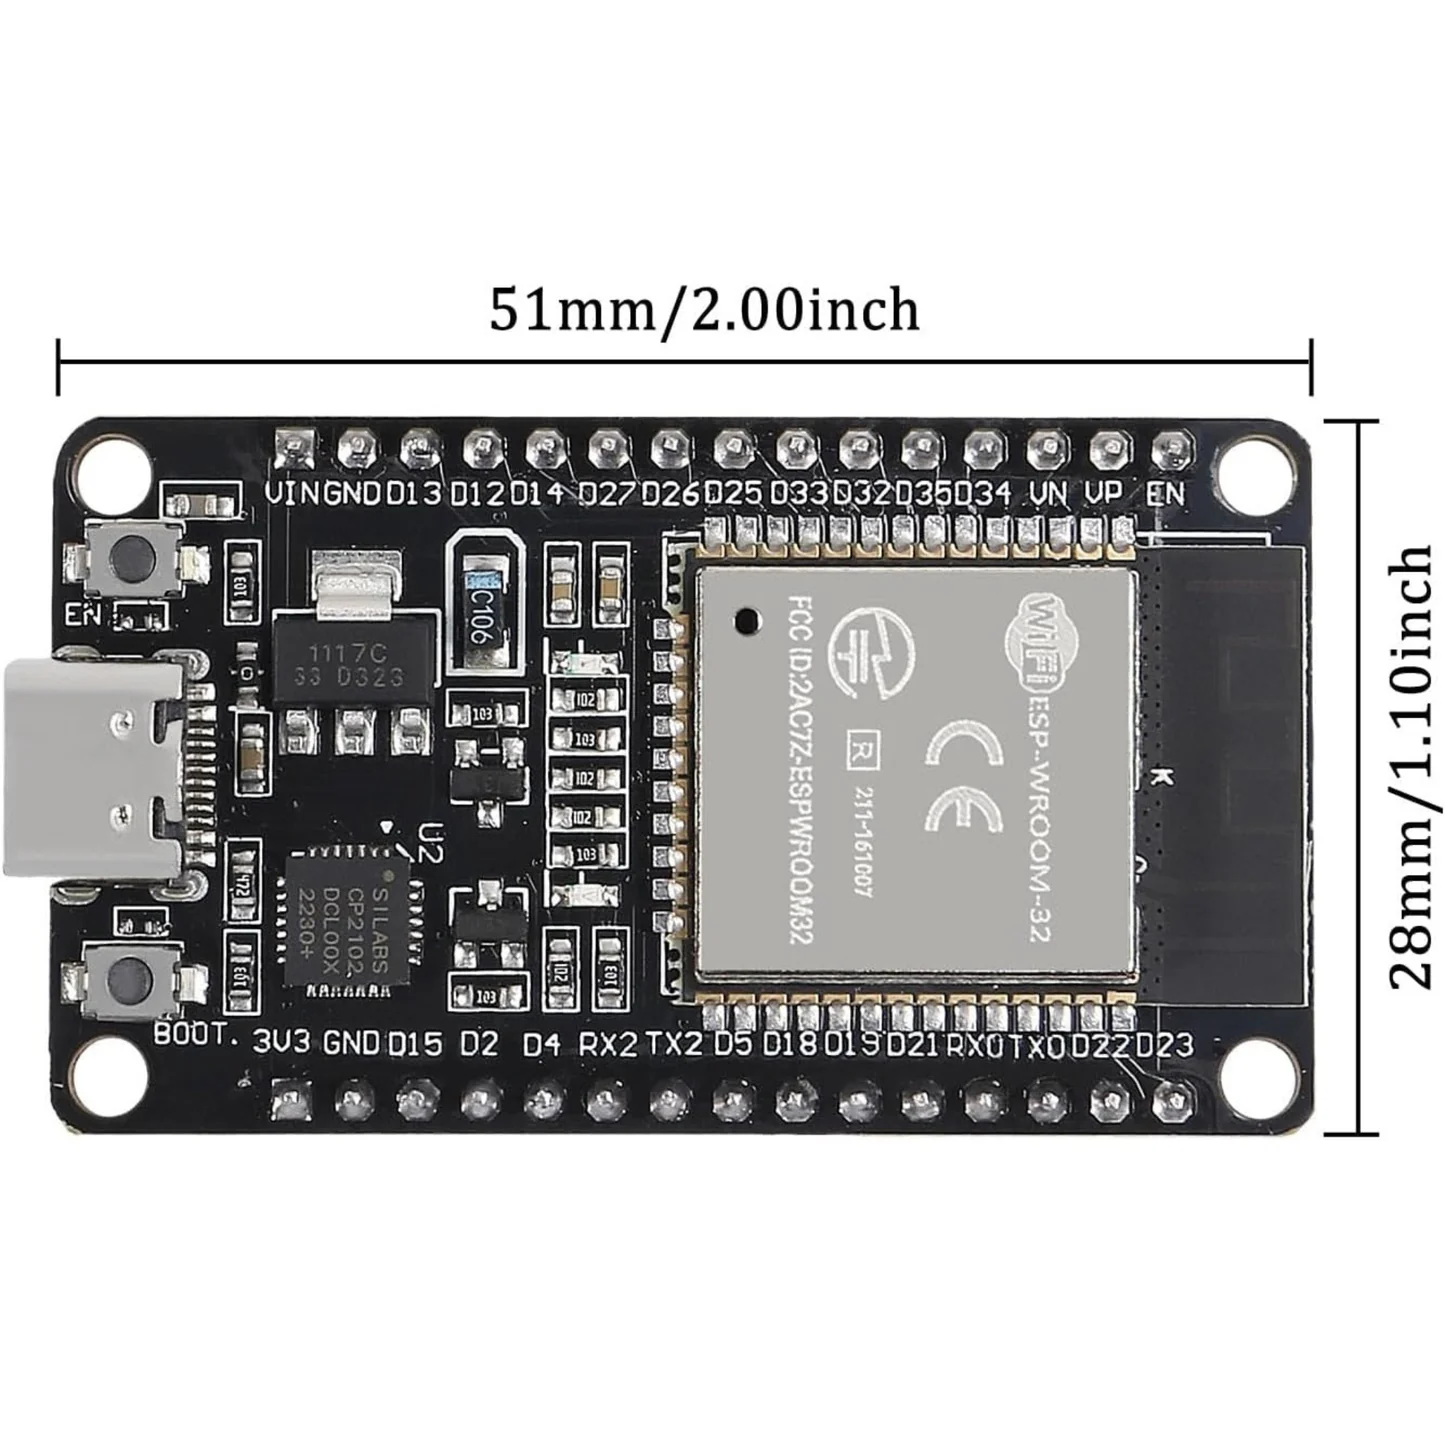
\includegraphics[width=0.6\textwidth]{assets/figures/esp32_devkit_v1.png}
    \caption{Dimensions du module ESP-32 DevKit V1}
    \label{fig:esp32_dimensions}
\end{figure}

\subsubsection{Efficacité énergétique}

D'après le datasheet de l'ESP-32, sa consommation électrique dépend fortement du mode de fonctionnement (veille, WiFi actif, Bluetooth actif, etc.).

\begin{figure}[H]
    \centering
    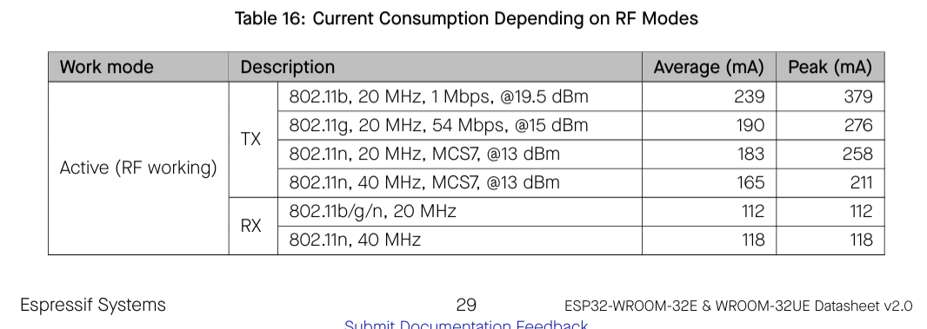
\includegraphics[width=0.75\textwidth]{assets/figures/esp32_consumption.png}
    \caption{Consommation énergétique de l'ESP-32 selon le mode de fonctionnement}
    \label{fig:esp32_power}
\end{figure}

\subsubsection{Communication sans fil}

Comme indiqué précédemment, l'ESP-32 inclut une antenne intégrée permettant la communication sans fil via WiFi et Bluetooth, offrant ainsi une grande flexibilité pour les applications connectées.

\begin{table}[H]
    \centering
    \begin{tabular}{|l|c|}
        \hline
        \textbf{Critère} & \textbf{Note (/10)} \\
        \hline
        Fréquence de travail & 9/10 \\
        \hline
        Taille & 7/10 \\
        \hline
        Efficacité énergétique & 7/10 \\
        \hline
        Communication sans fil & 8/10\\
        \hline
    \end{tabular}
    \caption{Résultats critères ESP-32 Devkit V1}
    \label{tab:esp32_results}
\end{table}

$$
\text{Note globale} = \frac{31}{50}
$$
\subsection{Raspberry Pi Pico W}

Le Raspberry Pi Pico W \cite{RaspberryPiPicoW} est une carte de développement basée sur le microcontrôleur RP2040, développée par la fondation Raspberry Pi. Il s'agit d'une évolution du Raspberry Pi Pico, à laquelle a été ajouté un module de communication sans fil.

Contrairement à des cartes plus complètes comme l'ESP-32 DevKit V1 \cite{ESP-32-Devkit-V1}, le Pico W ne dispose pas de Bluetooth, mais intègre une connectivité WiFi 2.4 GHz.

Cette carte peut être programmée en C/C++ via le SDK officiel, ainsi qu'en MicroPython, ce qui la rend accessible aussi bien pour le prototypage que pour des applications embarquées avancées.

\subsubsection{Fréquence de travail}

Le Raspberry Pi Pico W fonctionne jusqu'à une fréquence d'horloge de $133\,\si{\mega\hertz}$ grâce à son processeur double cœur ARM Cortex-M0+.

\subsubsection{Taille}

Les dimensions du module Raspberry Pi Pico W sont compactes, ce qui facilite son intégration dans des systèmes embarqués :

\begin{figure}[H]
    \centering
    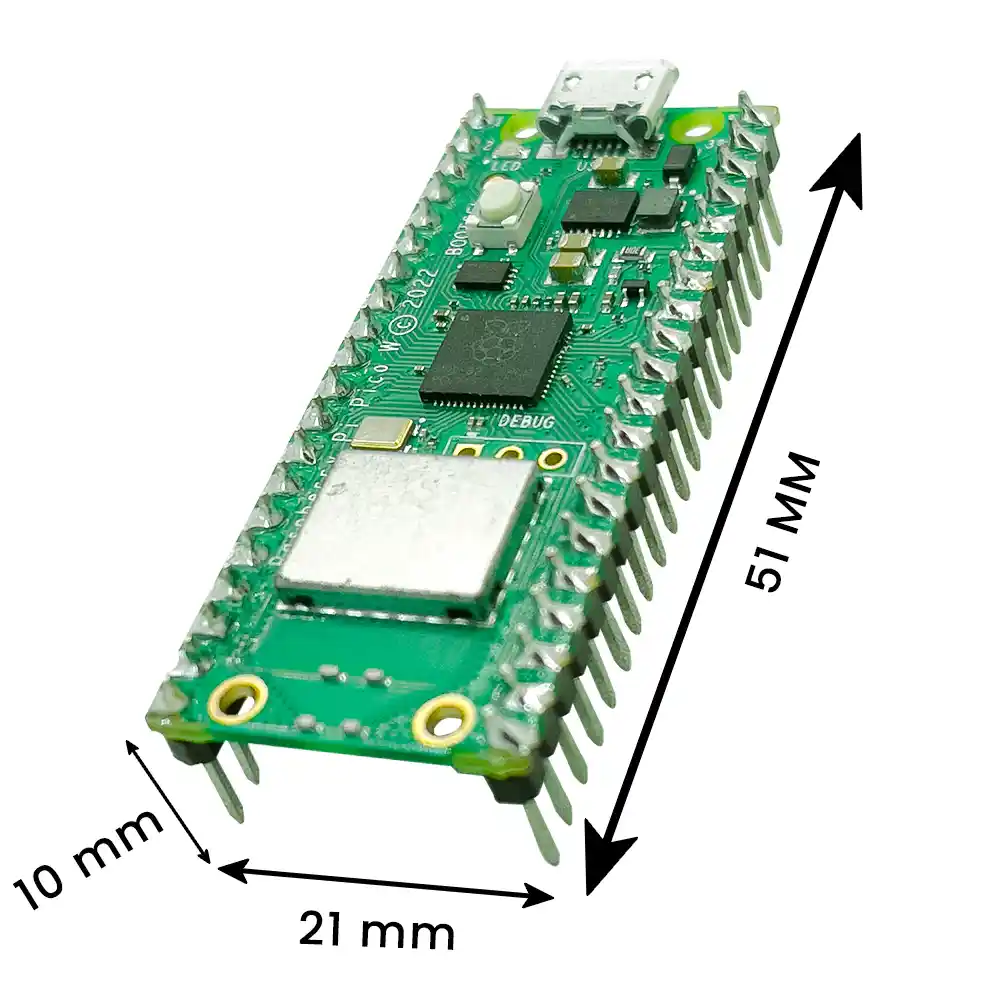
\includegraphics[width=0.6\textwidth]{assets/figures/raspberry_pico_w_dimensions.png}
    \caption{Dimensions du Raspberry Pi Pico W}
    \label{fig:pico_w_dimensions}
\end{figure}

\subsubsection{Efficacité énergétique}
Il est impossible de trouver avec précision une information relative à la consommation exacte de courant du module Raspberry Pico W. Cependant, en cherchant en ligne, voici ce que l'on peut trouver \href{https://stfn.pl/blog/34-pico-power-consumption-solar-panels/}{Raspberry Pico W Power consumption}.
Dans cette article, l'auteur décrit avoir observé un courant "continu" de $$0.45 \si\ampere$$ en ayant le wifi actif. Il ne s'agit bien entendu pas d'une mesure officielle du fabricant et il est donc nécessaire de la considérer avec suffisamment de recul.


\subsubsection{Communication sans fil}
Le Raspberry Pi Pico W intègre un module WiFi 2.4 GHz permettant la communication réseau. Toutefois, il ne supporte pas le Bluetooth, contrairement à certaines solutions concurrentes comme l'ESP32.

\begin{table}[H]
    \centering
    \begin{tabular}{|l|c|}
        \hline
        \textbf{Critère} & \textbf{Note (/10)} \\
        \hline
        Fréquence de travail & 7/10 \\
        \hline
        Taille & 9/10 \\
        \hline
        Efficacité énergétique & 8/10 \\
        \hline
        Communication sans fil & 6/10 \\
        \hline
    \end{tabular}
    \caption{Résultats critères Raspberry Pi Pico W}
    \label{tab:pico_results}
\end{table}

$$
\text{Note globale} = \frac{30}{50}
$$

\subsection{Choix final}

À l'issue de l'analyse comparative des deux microcontrôleurs étudiés (ESP-32 DevKit V1 et Raspberry Pi Pico W), le choix s'oriente vers l'ESP-32 DevKit V1.

Bien que le Raspberry Pi Pico W présente une meilleure efficacité énergetique et une taille inférieure à l'ESP, il reste limité par l'absence de Bluetooth ainsi que la fréquence d'horloge.

L'ESP-32 DevKit V1 se distingue par une meilleure polyvalence, notamment grâce à la présence du WiFi et du Bluetooth, une fréquence de travail plus élevée.


\section{IMU}
\subsection{Critères de choix}
\begin{table}[H]
    \centering
    \begin{tabular}{|c|l|}
        \hline
        \textbf{Critère} & \textbf{Justification} \\
        \hline
        Vitesse de lecture & Une lecture rapide des données permet une boucle de régulation plus rapide \\
        \hline
        Qualité du signal & Un signal bruité peut causer des problèmes dans la régulation \\
        \hline
        Taille & Comme le reste des composants, la taille du capteur doit être minimisée \\
        \hline
        Facilitée d'implémentation & Le capteur ne doit pas nécessiter des heures de travail d'implémentation\\
        \hline
        Prix & Le coût du capteur doit rester faible afin de limiter le coût total du robot. \\
        \hline
    \end{tabular}
    \caption{Critères de sélection de l'IMU}
    \label{tab:criteres_IMU}
\end{table}
\subsection{MPU6050}
Le premier candidat est le MPU6050, plus précisement la carte de développement GY-521 \cite{GY521_Datasheet}.
\subsubsection{Vitesse de lecture}
Les vitesse de lectures se trouvent dans le datasheet aux pages 12 et 13.
\begin{itemize}
    \item Fréquence max de lecture accéléromètre: 1 kHz;
    \item Fréquence max de lecture gyroscope:  8 kHz;
\end{itemize}
Les données sont accessibles via une interface I\textsuperscript{2}C simple à mettre en oeuvre \cite{MPU6050_Datasheet}.


\subsubsection{Qualité du signal}
Le capteur intègre un accéléromètre 3 axes et un gyroscope 3 axes 16 bits. 
Bien que plus ancien que les IMU récentes, il offre une qualité de mesure suffisante pour une estimation fiable de l'angle après application d'un filtre complémentaire software. Il n'intègre cependant pas de
filtrage de données embarqué.

\subsubsection{Taille}

\begin{figure}[H]
    \centering
    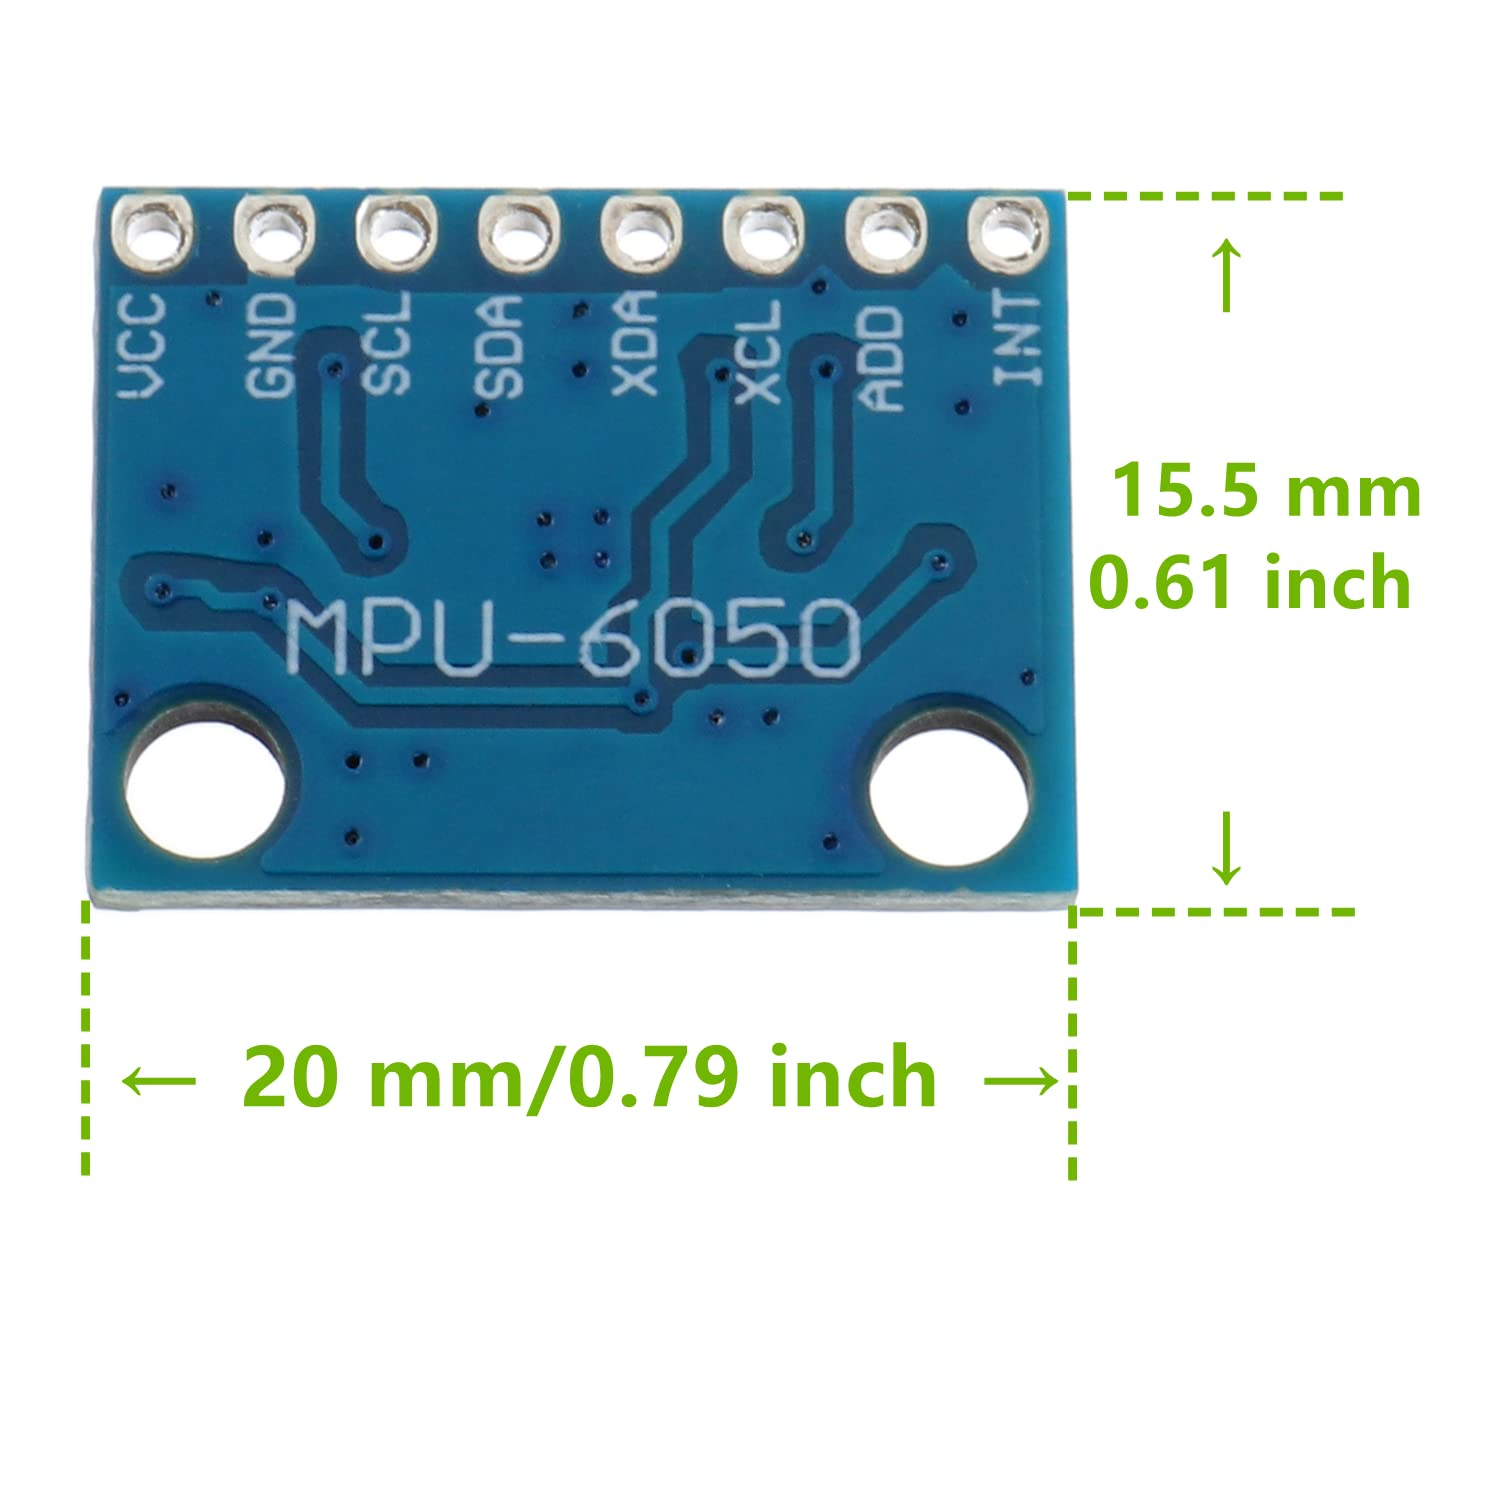
\includegraphics[width=0.6\textwidth]{assets/figures/mpu6050_dimensions.png}
    \caption{Dimensions de la carte GY-521}
    \label{fig:mpu_6050_dimensions}
\end{figure}


\subsubsection{Facilité d'implémentation}
Le MPU6050 est probablement l'IMU la plus documentée. De nombreuses bibliothèques Arduino et ESP-IDF existent, ce qui réduit fortement le temps de développement. 

\subsubsection{Prix}
Le module GY-521 basé sur le MPU6050 est très répandu et disponible chez de nombreux fournisseurs pour un prix compris entre 3 et 5 CHF. 
Son faible coût en fait une solution particulièrement intéressante pour les projets étudiants et les prototypes.
\begin{table}[H]
    \centering
    \begin{tabular}{|l|c|}
        \hline
        \textbf{Critère} & \textbf{Note (/10)} \\
        \hline
        Vitesse de lecture & 9/10 \\
        \hline
        Qualité du signal & 8/10 \\
        \hline
        Taille & 8/10 \\
        \hline
        Facilité d'implémentation & 10/10 \\
        \hline
        Prix & 10/10 \\
        \hline
    \end{tabular}
    \caption{Évaluation du MPU6050}
    \label{tab:mpu6050_resultats}
\end{table}

$$
\text{Note globale}=\frac{45}{50}
$$


\subsection{BMI160}

Le deuxième candidat est le BMI160, de chez Bosch.
\subsubsection{Vitesse de lecture}
Le BMI160 peut être paramétré afin d'offrir des fréquences de lectures variant de la manière suivante:
\begin{itemize}
    \item Gamme de fréquence de lecture accéléromètre: 12.5-1600 Hz;
    \item Gamme de fréquence de lecture gyroscope: 25-3200 Hz;
\end{itemize}
Le paramètrage se fait à l'aide des registres.

\subsubsection{Qualité du signal}
Grâce à une électronique plus récente, le BMI160 présente un bruit de mesure plus faible et une meilleure stabilité thermique que le MPU6050. 
Les mesures obtenues sont généralement plus précises.

\subsubsection{Taille}
\begin{figure}[H]
    \centering
    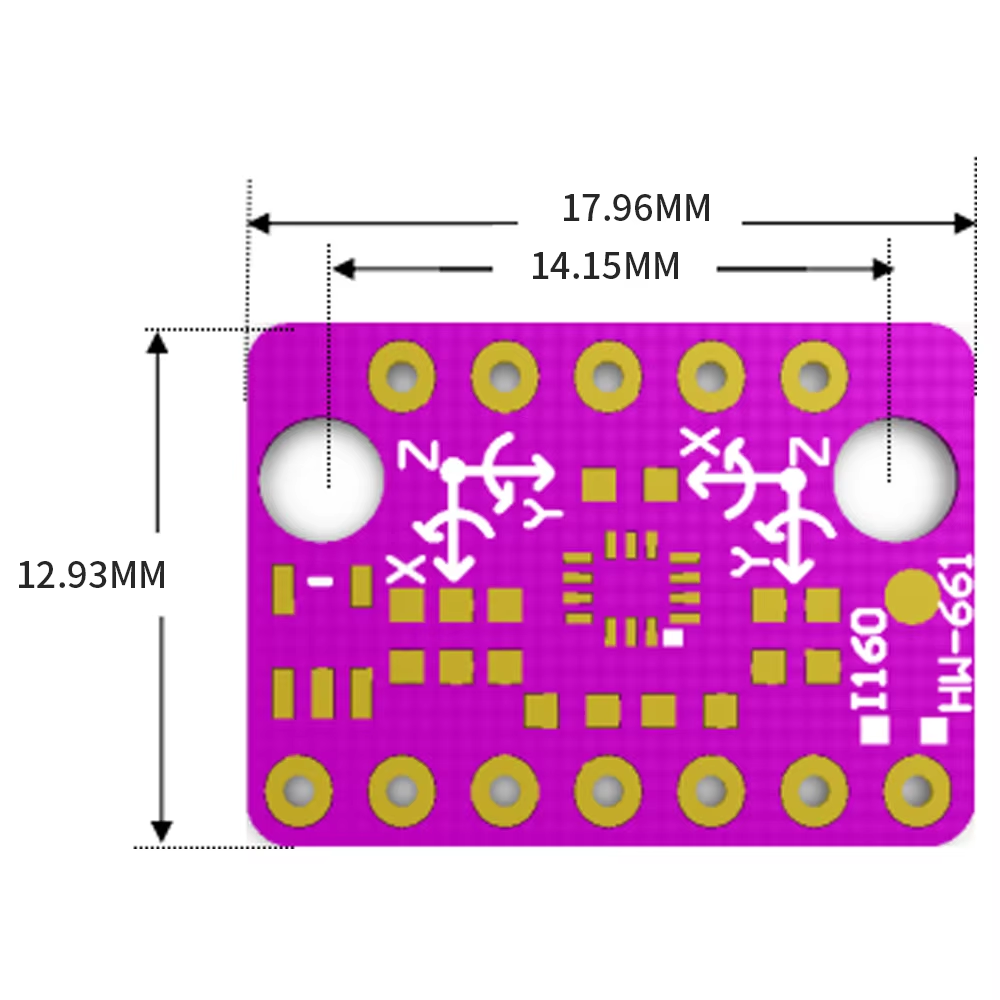
\includegraphics[width=0.6\textwidth]{assets/figures/bmi_160_dimensions.png}
    \caption{Dimensions du BMI160}
    \label{fig:bmi_160_dimensions}
\end{figure}

\subsubsection{Facilité d'implémentation}
Bien que plusieurs bibliothèques soient disponibles, le BMI160 nécessite une configuration plus complexe que le MPU6050. 
La documentation est également moins abondante au sein de la communauté des makers.

\subsubsection{Prix}

Les cartes de développement basées sur le BMI160 sont généralement vendues entre 6 et 10 CHF, soit environ deux fois plus cher qu'un module GY-521 intégrant le MPU6050.
\begin{table}[H]
    \centering
    \begin{tabular}{|l|c|}
        \hline
        \textbf{Critère} & \textbf{Note (/10)} \\
        \hline
        Vitesse de lecture & 10/10 \\
        \hline
        Qualité du signal & 9/10 \\
        \hline
        Taille & 9/10 \\
        \hline
        Facilité d'implémentation & 7/10 \\
        \hline
        Prix & 6/10 \\
        \hline
    \end{tabular}
    \caption{Évaluation du BMI160}
    \label{tab:bmi160_resultats}
\end{table}

$$
\text{Note globale}=\frac{41}{50}
$$
\subsection{Choix final}

Le BMI160 présente de meilleures performances en termes de qualité du signal et bénéficie d'une électronique plus récente. En revanche, ces avantages ne sont pas indispensables dans le cadre d'un robot auto-équilibré. Les performances du MPU6050 sont largement suffisantes pour atteindre la fréquence d'échantillonnage nécessaire et réaliser une estimation fiable de l'angle à l'aide d'un filtre logiciel.

Par ailleurs, le module GY-521 intégrant le MPU6050 est environ deux fois moins cher qu'une carte de développement basée sur le BMI160. Le grand nombre de bibliothèques disponibles et son faible coût permettent également de réduire le temps de développement ainsi que le coût global du projet.

Le choix s'est donc porté sur le \textbf{MPU6050}, qui offre le meilleur compromis entre performances, simplicité d'intégration et coût pour cette application.

\chapter{Principe physique}
Ce chapitre a pour objectif de présenter les principes physiques régissant le fonctionnement d'un robot auto-équilibrant. Avant de s'intéresser à la réalisation pratique du système, il est nécessaire d'établir un modèle théorique permettant de comprendre les phénomènes mis en jeu.

Le comportement du robot peut être assimilé à celui d'un pendule inversé. Ce système est naturellement instable : sans action extérieure, une perturbation provoque l'éloignement du système de sa position d'équilibre. Le rôle du système de commande est donc de générer un mouvement permettant de compenser en permanence cette instabilité.

Afin d'obtenir progressivement un modèle représentatif du robot réel, le système est étudié selon plusieurs niveaux de complexité. Dans un premier temps, le cas d'un pendule inversé simple est considéré. Ensuite, le déplacement horizontal du point d'appui est introduit à travers le modèle du pendule inversé monté sur un chariot. Finalement, les éléments propres au robot réel, tels que les moteurs et les roues, sont ajoutés.


\section{Pendule inversé}


\begin{figure}[H]
    \centering
    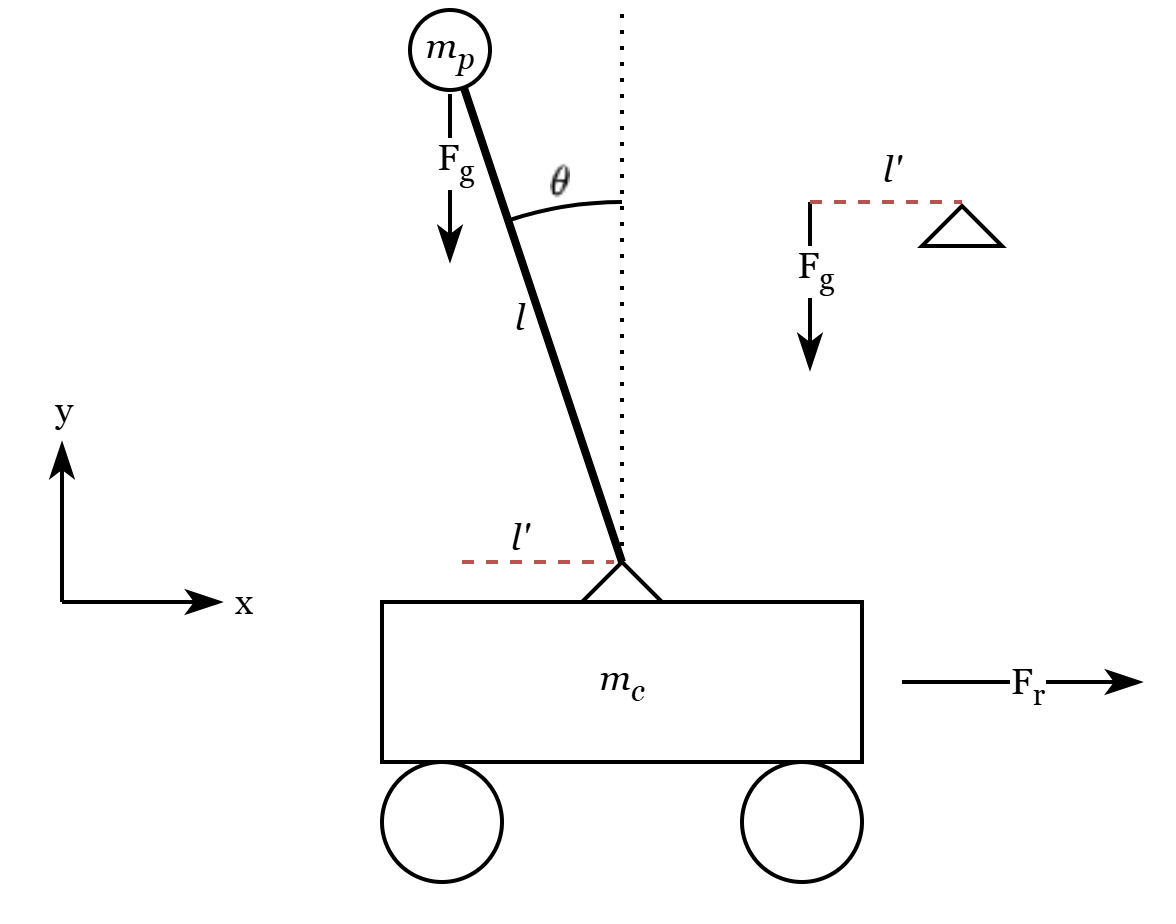
\includegraphics[width=0.8\textwidth]{assets/schemas/pendule_inverse.png}
    \caption{Modèle du pendule inversé sur chariot}
    \label{fig:pendule_chariot}
\end{figure}

Le schéma \ref{fig:pendule_chariot} représente le pendule inversé avec un chariot. D'abord, le chariot est considéré comme immobile afin de simplifier l'étude du système. Le pendule est donc assimilé à une tige rigide de longueur $l$ portant une masse ponctuelle $m_p$, libre de tourner autour d'un pivot sans frottement.

Le principe fondamental de la dynamique en rotation s'écrit :

\begin{equation}
\sum T = J_b\ddot{\theta}
\end{equation}

où :

\begin{itemize}
    \item $T$ est la somme des moments (couples) appliqués au point de rotation (triangle sur le schéma);
    \item $J_b$ est le moment d'inertie du pendule par rapport au pivot ;
    \item $\ddot{\theta}$ est l'accélération angulaire.
\end{itemize}

Le seul effort appliqué au pendule est son poids

\begin{equation}
\vec{F_g}=m_p\vec{g}
\end{equation}

La réaction du pivot passe par le point de rotation et ne génère donc aucun moment.

Le couple généré par le poids par rapport au pivot vaut

\begin{equation}
T_p = m_pgl\sin(\theta)
\end{equation}

Le moment d'inertie d'une masse ponctuelle située à une distance $l$ du pivot est

\begin{equation}
J_b = m_pl^2.
\end{equation}

En appliquant le principe fondamental de la dynamique en rotation, on obtient

\begin{equation}
m_pgl\sin(\theta)=m_pl^2\ddot{\theta}.
\end{equation}

Après simplification,

\begin{equation}
\boxed{\ddot{\theta}=\frac{g}{l}\sin(\theta)}
\end{equation}

Cette équation est non linéaire en raison de la présence du terme $\sin(\theta)$.

Dans le cas de faibles inclinaisons, l'approximation

\begin{equation}
\sin(\theta)\approx\theta
\end{equation}

permet d'obtenir l'équation linéarisée

\begin{equation}
\boxed{\ddot{\theta}=\frac{g}{l}\theta.}
\end{equation}

Cette équation met en évidence l'instabilité du pendule inversé. En effet, contrairement au pendule classique dont l'équation est

\begin{equation}
\ddot{\theta}+\frac{g}{l}\theta=0,
\end{equation}

le signe positif devant le terme en $\theta$ implique que toute perturbation s'amplifie avec le temps. Le système est donc marginalement stable, ce qui signifie qu'il admet un seul point de stabilité, ($\theta = 0$), dans la réalité, il peut être considéré comme instable.

\section{Pendule inversé avec chariot}

Le modèle précédent possède cependant une limitation importante : le point d'appui est fixe. Dans le cas d'un robot auto-équilibrant, le point de contact avec le sol peut se déplacer grâce aux roues.

Le modèle du pendule inversé monté sur un chariot permet de représenter ce comportement. Le chariot de masse $m_c$ peut se déplacer horizontalement selon l'axe $x$, tandis que le pendule de masse $m_p$ peut tourner autour de son point d'attache.

Les deux degrés de liberté du système sont donc :

\begin{itemize}
    \item la position horizontale du chariot $x$ ;
    \item l'angle du pendule $\theta$.
\end{itemize}

La dérivation des équations de Lagrange n'est pas présentée dans ce rapport, cette méthode n'ayant pas été abordée dans le cadre de la formation suivie. Les équations utilisées proviennent de la littérature et ont été adaptées au modèle étudié. Une référence est fournie pour le lecteur souhaitant approfondir cette méthode.
\cite{wiki_inverted_pendulum}
Voici donc les équations proposées pour ce modèle.
\begin{equation}
(m_c+m_p)\ddot{x}
+
m_pl\ddot{\theta}\cos(\theta)
-
m_pl\dot{\theta}^{2}\sin(\theta)
=
F_r
\end{equation}

\begin{equation}
m_pl\ddot{x}\cos(\theta)
+
m_pl^2\ddot{\theta}
-
m_pgl\sin(\theta)
=
0
\end{equation}

où $F_r$ représente la force appliquée au chariot.

Ces équations montrent le couplage entre le mouvement horizontal du chariot et la rotation du pendule. Une accélération du chariot provoque une variation de l'angle du pendule, qui doit être compensée par une commande adaptée.

\section{Modèle avec moteurs et roues}

Le modèle du pendule sur chariot constitue une bonne approximation du fonctionnement du robot. Cependant, le déplacement du chariot est remplacé dans le système réel par la rotation de deux roues entraînées par des moteurs pas à pas.

Le modèle complet doit alors au moins intégrer :

\begin{itemize}
    \item la masse et l'inertie du châssis ;
    \item l'inertie des roues ;
    \item le couple fourni par les moteurs.
\end{itemize}

La prise en compte de ces différents éléments conduit à un modèle mécanique plus complexe. Les équations obtenues nécessitent l'utilisation des équations de Lagrange appliquées à un système comportant plusieurs degrés de liberté. Cette méthode permet de prendre en compte les interactions entre le mouvement de translation du robot et la rotation du pendule.

La dérivation complète de ces équations dépasse le cadre de ce rapport et fait intervenir des notions de mécanique analytique qui n'ont pas été abordées dans le cursus suivi. Les équations utilisées dans cette section proviennent donc de la littérature, notamment du travail réalisé par l'\Gls{eth} \cite{eth_two_w}.

Les équations obtenues sont les suivantes :

\begin{equation}
\ddot{x}
=
\frac{1}{d_1}
\left(
a I_O \dot{\theta}^{2}\sin(\theta)
-
a^2 g \sin(\theta)\cos(\theta)
+
T
\left(
\frac{I_O}{r}
+
a\cos(\theta)
\right)
\label{eq:ddx}
\right)
\end{equation}

\begin{equation}
\ddot{\theta}
=
\frac{1}{d_1}
\left(
-a^2 \dot{\theta}^{2}\sin(\theta)\cos(\theta)
+
a m_O g\sin(\theta)
-
T
\left(
m_O
+
\frac{a}{r}\cos(\theta)
\right)
\right)
\label{eq:ddtheta}
\end{equation}

où $\ddot{x}$ représente l'accélération horizontale du robot et $\ddot{\theta}$ l'accélération angulaire du châssis par rapport à la verticale. Le terme $T$ correspond au couple appliqué par les moteurs sur les roues. Celui-ci constitue l'entrée de commande du système et permet d'agir sur l'équilibre du robot.

Les termes liés à la masse et à l'inertie permettent de représenter l'influence des différents éléments mécaniques. La masse du châssis est représentée par $m_b$, tandis que $m_w$ correspond à la masse d'une roue. Les moments d'inertie $J_b$ et $J_w$ représentent respectivement l'inertie du châssis et des roues autour de leur centre de masse.

Les simplifications suivantes sont utilisées afin de regrouper certains paramètres et de rendre les équations plus lisibles :

\begin{equation}
\begin{aligned}
a &= m_b l \\
I_O &= J_b + m_b l^2 \\
m_{\mathrm{tot}} &= m_b + 2m_w \\
m_O &= m_{\mathrm{tot}} + \frac{J_w}{r^2} \\
d_1 &= I_O m_O - a^2\cos^2(\theta)
\end{aligned}
\end{equation}

Le paramètre $r$ représente le rayon des roues. Le terme $\frac{J_w}{r^2}$ permet de ramener l'inertie de rotation des roues sous la forme d'une masse équivalente lors du mouvement de translation du robot.

Le terme $d_1$ représente le dénominateur commun des équations du mouvement et traduit le couplage entre les différents éléments mécaniques du système. Sa dépendance en fonction de $\theta$ montre que la dynamique du robot varie en fonction de son inclinaison.

Ce modèle fournit ainsi une représentation plus fidèle du comportement du robot réel. Il permet notamment d'étudier l'influence des paramètres mécaniques sur la dynamique du système et constitue une base pour le développement de la loi de commande.

La différence principale entre le modèle incluant les roues et les modèles précédents réside dans l'apparition du terme associé au couple moteur dans l'équation de la dynamique angulaire du levier. Contrairement aux modèles simplifiés, l'actionneur intervient directement dans l'équilibre des moments autour de l'axe de rotation.

Le couple appliqué aux roues génère un moment opposé aux effets gravitationnels agissant sur le centre de masse du levier. Il constitue ainsi une action corrective permettant de réduire l'écart angulaire par rapport à la position d'équilibre. 

Le couple moteur agit également par l'intermédiaire de l'accélération horizontale du robot : le mouvement des roues provoque une réaction inertielle qui modifie la dynamique du levier. Les deux effets contribuent donc conjointement à la stabilisation du système. Le couple moteur représente ainsi l'entrée de commande permettant de compenser le moment gravitationnel et de maintenir le robot autour de sa position d'équilibre.
\chapter{Mécanique}
\label{chap:mecanique}
\begin{figure}[H]
    \centering
    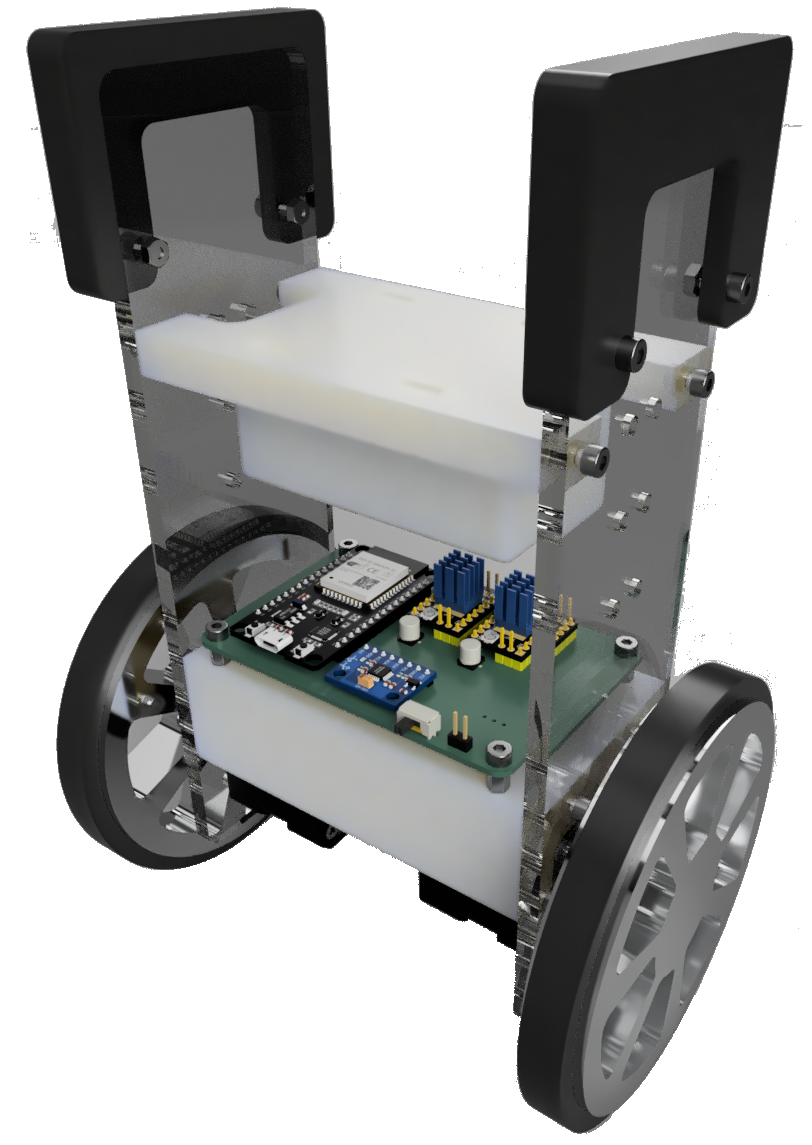
\includegraphics[width=0.8\textwidth]{assets/figures/meca_raytracing.png}
    \caption{Maquette 3D, raytracée}
    \label{fig:meca_raytraced}
\end{figure}

Une fois le principe physique expliquée, il est temps de réaliser la maquette. Le but ici est de tenir compte des reflexions faites durant la partie théorique.

Dans ce chapitre, l'entiereté de la conception mécanique de la maquette sera traitée en commençant par les outils utilisés, en traitant ensuite des contraintes mécaniques connues.

Finalement, une rapide instruction de montage sera présentée.

L'ensemble des dessins mécanique se trouvent à l'annexe \ref{annexe:dessins_mecaniques}. De plus, les fichiers 3D des pièces se trouvent également sur le Git indiqué en annexe \ref{annexe:git}.

\section{Méthode et outils}
\subsection{Logiciels}

La conception mécanique du robot a été réalisée à l'aide du logiciel Fusion360 de Autocad. Cette étape a permis de modéliser l'ensemble des composants du robot avant leur fabrication, de vérifier leur intégration ainsi que d'anticiper les éventuels problèmes d'assemblage.

L'utilisation d'un modèle tridimensionnel présente plusieurs avantages. Elle permet notamment de contrôler les dimensions de l'ensemble, de vérifier les interfaces entre les différents composants, d'optimiser la répartition des masses et de préparer la fabrication des différentes pièces.

Le PCB ayant été réalisé en premier, ce deriner a été importé dans le modèle afin de pouvoir l'intégrer directement au dessin 3D.
\subsection{Outillage}

Essentiellement, le robot est constitué de pièces imprimées en 3D ainsi que de pièces découpées au laser. Divers éléments d'assemblage (vis, colonnettes, écrous, etc.) proviennent du MakeLab ou de l'atelier mécanique.

Les pneus ainsi que les protections anti-chutes ont été imprimé en TPU, un filament flexible afin d'améliorer l'adhérance et amortir l'impact d'une éventuelle chute.

Le tableau \ref{tab:machines} répertorie l'ensemble des machines utilisées pour la fabrication de la maquette.

\begin{table}[H]
\centering
\begin{tabular}{|c|p{6cm}|c|}
\hline
\textbf{Machine} & \textbf{Emplacement} & \textbf{Technologie} \\
\hline
Prusa Core One & MakeLab & \acrshort{fdm} \\
\hline
CNC 3 axes & Centre de formation des polymécaniciens, Payerne & Usinage CNC \\
\hline
Découpeuse laser & MakeLab & Découpe laser \\
\hline
BambuLab V1 & MakeLab & \acrshort{fdm}, TPU \\
\hline
\end{tabular}
\caption{Machines utilisées pour la fabrication de la maquette}
\label{tab:machines}
\end{table}

\section{Contraintes mécaniques}

Avant de débuter la conception du châssis, plusieurs contraintes mécaniques ont été identifiées soit par le cahier des charges, soit par le chapitre \ref{chap:principe_physique}.

Les principales contraintes sont les suivantes :

\begin{itemize}
    
    \item assurer une rigidité suffisante afin de limiter les déformations du châssis ;
    \item assurer un positionnement du centre de gravité "variable" ;
    \item limiter la masse totale du robot ; 
    \item garantir un encombrement réduit tout en conservant un accès aisé aux composants ;
    \item permettre un montage et un démontage simples des différents éléments ;
    \item prévoir un passage des câbles limitant les risques d'arrachement ou de frottement avec les parties mobiles.
\end{itemize}

Ces contraintes ont servi de fil conducteur durant toute la phase de conception mécanique.


\subsection{Centre de gravité}

Le centre de gravité constitue un élément essentiel dans la conception d'un robot auto-équilibrant. Contrairement à un robot classique, la stabilité dépend directement de la position de la masse par rapport à l'axe des roues.

Un centre de gravité situé plus haut augmente le bras de levier entre la masse et les roues. Le robot bascule alors plus lentement, ce qui laisse davantage de temps au correcteur pour réagir. En revanche, cette configuration nécessite un déplacement plus important des roues pour maintenir l'équilibre.

À l'inverse, un centre de gravité trop bas rend le système beaucoup plus réactif mais également plus difficile à stabiliser, les variations d'angle étant plus rapides.

C'est pour cette raison que plusieurs perçage ont été réalisés sur les plaques en PVC se situant sur les côtés, de cette manière, la batterie peut être déplacée afin de modifier les caractéristiques du robot.

\subsection{Rigidité}

Le châssis doit présenter une rigidité suffisante afin que les mouvements du robot correspondent fidèlement aux mesures fournies par l'unité de mesure inertielle (IMU).

Une structure trop flexible pourrait engendrer des vibrations ou des déformations susceptibles de perturber les mesures d'accélération et de vitesse angulaire, ce qui dégraderait les performances du système d'équilibrage.
\subsection{Masse}

La masse du robot influence directement le couple que doivent fournir les moteurs ainsi que la consommation électrique.

Dans cette optique, les matériaux utilisés dans la fabrication du châssis ne sont pas massique, à l'exception des roues, (voir\ref{subsection:roues}).

\subsection{Encombrement}

Les dimensions du robot ayant été indiquées par le cahier des charges, voici les dimensions obtenues.

156x143x248mm

L'implantation des différents modules a également été étudiée afin de faciliter l'assemblage, la maintenance ainsi que le passage des câbles. Une attention particulière a été portée à l'accessibilité des principaux éléments, notamment la batterie, le switch d'alimentation et les connecteurs.

\subsection{Roues}
\label{subsection:roues}

Le choix des roues joue un rôle important dans le comportement dynamique du robot. Leur diamètre détermine notamment la vitesse linéaire obtenue pour une vitesse de rotation donnée des moteurs, tandis que leur masse influence directement leur moment d'inertie.

Une roue présentant un moment d'inertie élevé nécessite davantage de couple pour accélérer ou ralentir. Cette caractéristique peut modifier la réactivité du système d'équilibrage et influencer les performances de la régulation.

Afin d'évaluer expérimentalement cet effet, deux jeux de roues de géométrie identique ont été réalisés : un premier en aluminium et un second en plastique PLA. Les roues peuvent être interchangeées sans modification de la structure du robot, ce qui permet de comparer directement l'influence de leur masse et de leur moment d'inertie sur le comportement du système.

\section{Assemblage}
Le chassis est assemblé moyennant des vis, écrous et inserts M3.

\section{Caractéristiques}


\begin{figure}[H]
    \centering
    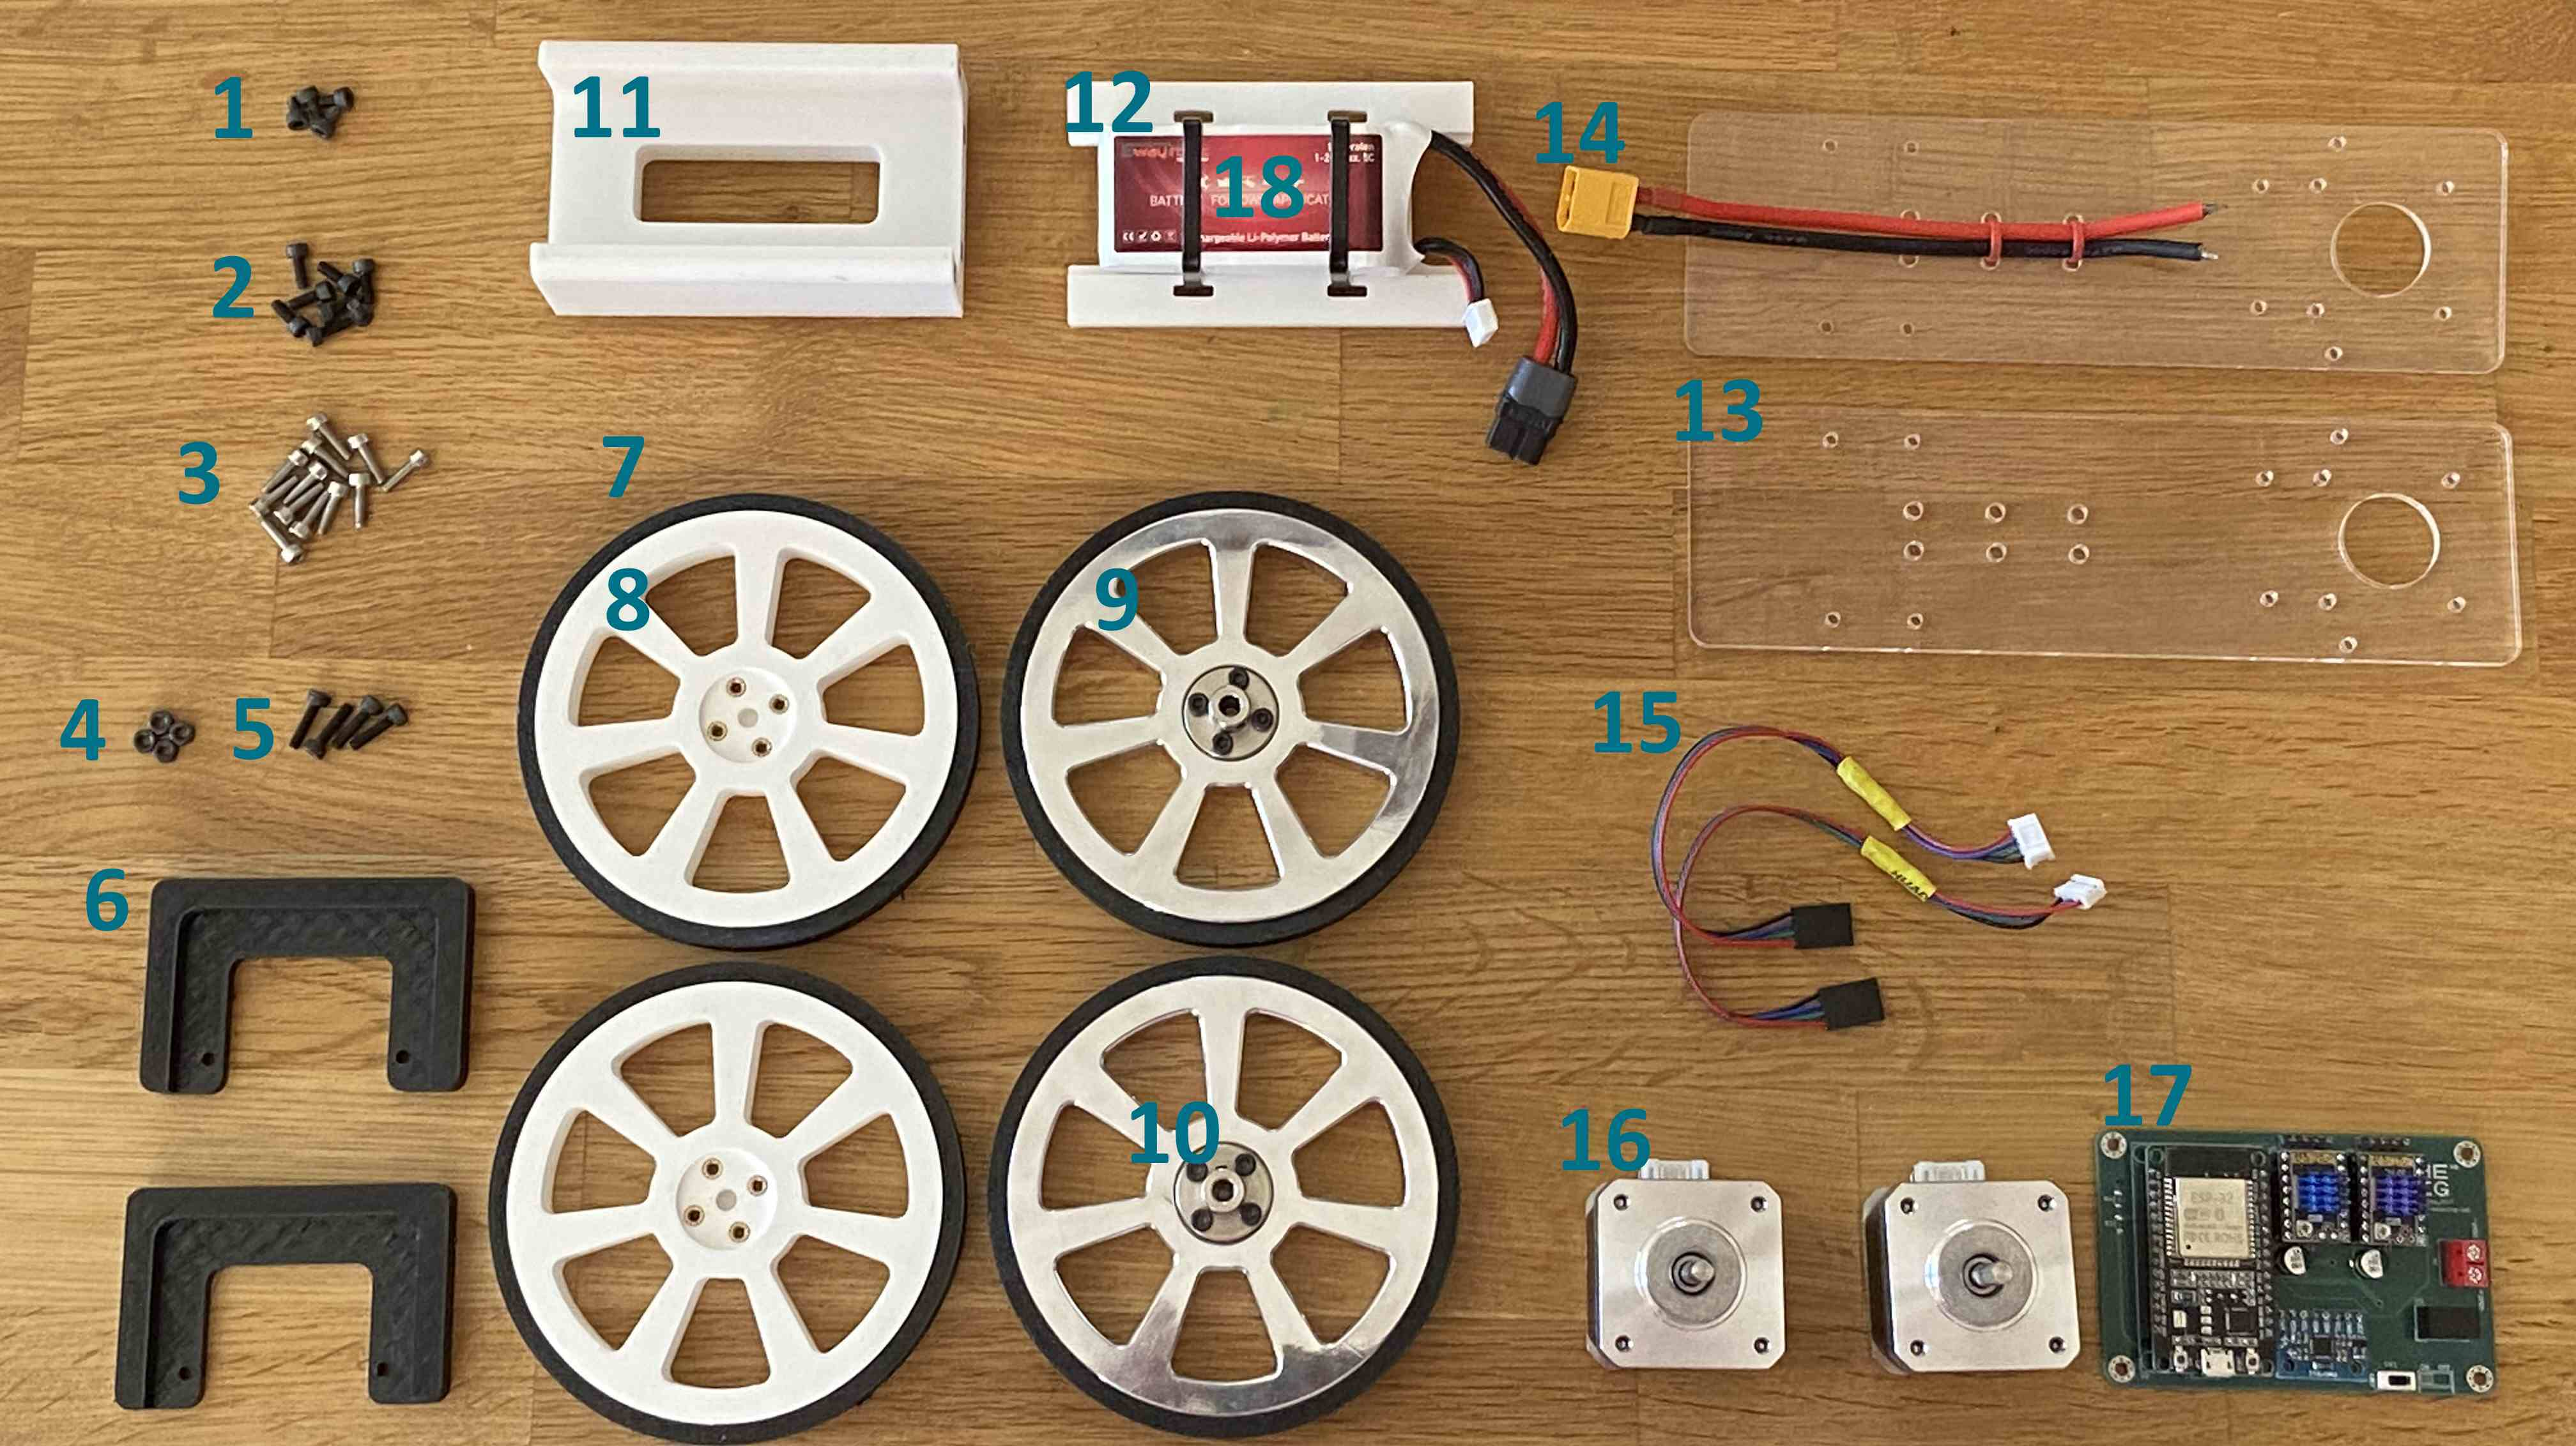
\includegraphics[width=1\textwidth]{assets/figures/all_pieces.jpg}
    \caption{Ensemble des pièces composant la maquette}
    \label{fig:all_pieces}
\end{figure}

Le tableau \ref{tab:masse_pieces} présente les masses individuelles des composants identifiés sur la figure \ref{fig:all_pieces}. Les masses des vis, écrous et inserts M3 sont négligées dans les calculs, leur contribution étant faible devant la masse totale de la maquette.
Les résultats sont donnés en \si{\kilogram}.
\begin{table}[H]
\centering
\begin{tabular}{|c|p{6cm}|c|c|c|}
\hline
\textbf{Pièce} & \textbf{Désignation} & \textbf{Mesure} & \textbf{Fusion360} & \textbf{Unité} \\
\hline
6 & Protection anti-chute & $0.010$ & -- & \si{\kilogram} \\
\hline
7 & Pneu & $0.013$ & $0.014$ & \si{\kilogram} \\
\hline
8 & Jante PLA & $0.035$ & $0.030$ & \si{\kilogram} \\
\hline
9 & Jante ALU & $0.163$ & 0.163& \si{\kilogram} \\
\hline
10 & Coupleur avec vis de montage & $0.013$ & $0.010$ & \si{\kilogram} \\
\hline
11 & Support PCB & $0.047$ & $0.047$ & \si{\kilogram} \\
\hline 
12 & Support batterie& $0.018$ & $0.018$ & \si{\kilogram} \\
\hline
13 & Plaque latérale & $0.065$ & $0.065$ & \si{\kilogram} \\
\hline
14 & Câble d'alimentation & $0.016$ & $-$ & \si{\kilogram} \\
\hline
15 & Câble moteur & $0.000$ & $-$ & \si{\kilogram} \\
\hline
16 & Moteur pas à pas & $0.281$ & 0.281 & \si{\kilogram} \\
\hline
17 & PCB & $0.045$ & 0.045& \si{\kilogram} \\
\hline
18 & Batterie & $0.150$ & 0.150 & \si{\kilogram} \\
\hline
\end{tabular}
\caption{Masses des différentes pièces composant la maquette.}
\end{table}
\label{tab:masse_pieces}

A partir des masses individuelles et des propriétés géométriques obtenues par Fusion360, les paramètres mécaniques nécessaires à la modélisation dynamique (voir \ref{chap:principe_physique}) sont déterminés.

La masse totale des sous-ensembles est obtenue à l'aide d'une nouvelle mesure.

Les moments d'inertie sont directement extraits de Fusion360 à partir de l'outil d'analyse des propriétés de masse. Le calcul est effectué autour du centre de masse du sous-ensemble considéré et selon l'axe de rotation correspondant. Pour les roues, le moment d'inertie $J_w$ est calculé autour de l'axe de rotation de la roue. Pour le châssis, le moment $J_b$ correspond au moment d'inertie autour de l'axe des roues, après exclusion des masses tournantes.

La distance $l$ entre l'axe des roues et le centre de masse est également déterminée à partir de la position du centre de gravité calculée par Fusion360.
\begin{table}[H]
\centering
\begin{tabular}{|l|c|p{5.2cm}|c|c|}
\hline
\textbf{Symbole} & \textbf{Origine} & \textbf{Définition} & \textbf{Valeur} & \textbf{Unité} \\
\hline
$m_b$ & Mesure & Masse du châssis & $1.018$ & \si{\kilogram} \\
\hline
$m_w$ & Mesure & Masse d'une roue complète (coupleur, jante ALU et pneu) & $0.195$ & \si{\kilogram} \\
\hline
$-$ & Mesure & Masse d'une roue complète (coupleur, jante PLA et pneu) & $0.083$ & \si{\kilogram} \\
\hline
$l$ & Fusion360 & Distance entre l'axe des roues et le centre de masse & $0.0344$ & \si{\metre} \\
\hline
$r$ & Mesure & Rayon de la roue & $0.055$ & \si{\metre} \\
\hline
$J_w$ & Fusion360 & Moment d'inertie d'une roue (ALU) autour de son axe de rotation & $2.522\times10^{-4}$ & \si{\kilogram\metre\squared} \\
\hline
$-$ & Fusion360 & Moment d'inertie d'une roue (PLA) autour de son axe de rotation & $7.615\times10^{-5}$ & \si{\kilogram\metre\squared} \\
\hline
$J_b$ & Fusion360 & Moment d'inertie du châssis (sans les roues) autour de l'axe des roues & $4.021\times10^{-3}$ & \si{\kilogram\metre\squared} \\
\hline
\end{tabular}
\caption{Caractéristiques mécaniques de la maquette utilisées dans la modélisation.}
\label{tab:caracteristiques_mecaniques}
\end{table}

L'analyse du modèle CAO réalisée sous Fusion 360 permet de déterminer avec précision la position de l'\acrshort{imu} par rapport à l'axe de rotation des roues. Cette information est nécessaire pour tenir compte des accélérations linéaires mesurées par le capteur lors des mouvements du robot.

La position de l'\acrshort{imu} est exprimée en coordonnées polaires, définies par la distance $\rho$ entre le capteur et l'axe de rotation, ainsi que par l'angle $\phi$ :

$$
\phi = -0.373~\mathrm{rad}
$$

$$
\rho = 51.13~\mathrm{mm}
$$

\chapter{Electronique}
Cette partie décrit l'architecture électronique mise en œuvre dans le cadre du projet. Elle présente l'ensemble des choix de conception réalisés afin d'assurer l'alimentation, le contrôle et l'actionnement de la maquette, tout en respectant les contraintes électriques et fonctionnelles identifiées.

L'architecture globale du système est d'abord introduite au moyen d'un schéma bloc, permettant de mettre en évidence les différents sous-ensembles et leurs interactions. Les solutions retenues pour la distribution d'énergie ainsi que pour l'entraînement des moteurs sont ensuite détaillées, en particulier au regard des contraintes de courant et de dimensionnement des composants.

Une attention particulière est portée au choix du microcontrôleur, élément central du système de commande, ainsi qu'à l'implémentation de l'électronique de puissance associée aux drivers moteurs. Enfin, la réalisation du schéma électrique complet, le prototypage sur breadboard et la conception du \gls{pcb} sont présentés et justifiés.
\section{Alimentation}
\section{Schéma bloc}
\section{Drivers moteurs}
\subsection{Courant max}
\section{Microcontrôleur}
\section{Schéma électrique}
\section{Breadboard}
\section{\gls{pcb}}



\chapter{Programmation}
\section{Outils utilisés}
\section{Algorithme}
\section{Drivers moteurs}
\section{IMU}
\chapter{Mesures}
\section{Méthode}
\subsection{Appareils de mesure}

\begin{table}[H]
    \centering
    \begin{tabular}{|l|l|l|}
        \hline
        \textbf{Type} & \textbf{Marque} & \textbf{Modèle} \\
        \hline
        Multimètre numérique & UNI-T & UT61E \\
        \hline
    \end{tabular}
    \caption{Appareils de mesure}
    \label{tab:appareils_mesure}
\end{table}


\section{Batterie}

Afin de mesurer correctement le niveau de la batterie, un pont diviseur est utilisé, comme expliqué dans le chapitre consacré à la maquette.

Il est important de s'assurer que les résistances utilisées dans le pont diviseur sont correctement reportées dans le code afin de garantir une lecture fidèle de la tension de la batterie.

\begin{table}[H]
    \centering
    \begin{tabular}{|l|c|c|}
        \hline
        \textbf{Symbole} & \textbf{Valeur théorique} & \textbf{Valeur mesurée} \\
        \hline
        R4 & 10 k$\Omega$ & 10.12 k$\Omega$ \\
        \hline
        R3 & 51 k$\Omega$ & 49.50 k$\Omega$ \\
        \hline
    \end{tabular}
    \caption{Mesure du pont diviseur}
    \label{tab:mesure_pont_diviseur}
\end{table}

 À l'aide des valeurs mesurées, le nouveau rapport du pont diviseur peut être calculé puis introduit dans le code afin d'affiner la mesure de la tension de la batterie.

Le rapport théorique du pont diviseur est donné par :

$$
\frac{R_3+R_4}{R_4}
$$

En utilisant les valeurs mesurées, on obtient :

$$
\frac{50.82 + 10.12}{10.12}=6.022
$$

Le rapport théorique valait :

$$
\frac{51+10}{10}=6.10
$$

On constate donc un écart d'environ (1\%) entre le rapport théorique et le rapport réel.

Il est alors possible de corriger les constantes utilisées dans le programme en remplaçant les valeurs nominales des résistances par les valeurs mesurées :


Le facteur de conversion utilisé pour reconstruire la tension de la batterie devient alors :

$$
\frac{50820+10120}{10120}=6.022
$$

Cette correction permet d'améliorer la précision de la mesure de la tension et de réduire l'erreur introduite par les tolérances des résistances du pont diviseur.

\section{Tensions, Courants}
Afin de mesurer la consommation énergétique de la maquette, l'idée est de réaliser une mesure du courant total dans le système.
Pour ce faire, le multimètre est placé en mode ampèremètre entre le connecteur de la batterie et celui du PCB.

\begin{table}[H]
    \centering
    \begin{tabular}{|l|c|c|}
        \hline
        \textbf{Grandeur mesurée} & \textbf{Valeur théorique} & \textbf{Valeur mesurée} \\
        \hline
        $V_{bat}$ & - & 16.48 V \\
        \hline
        $V_{IO}$ & 3.3 V & 3.28 V \\
        \hline
        $I_{tot}$ & - & 0.5 A \\
        \hline
    \end{tabular}
    \caption{Mesures électriques - Moteurs allumés}
    \label{tab:moteurs_allumes}
\end{table}

\begin{table}[H]
    \centering
    \begin{tabular}{|l|c|c|}
        \hline
        \textbf{Grandeur mesurée} & \textbf{Valeur théorique} & \textbf{Valeur mesurée} \\
        \hline
        $V_{bat}$ & - & 16.52 V \\
        \hline
        $V_{IO}$ & 3.3 V & 3.28 V \\
        \hline
        $I_{tot}$ & - & 0.5 A \\
        \hline
    \end{tabular}
    \caption{Mesures électriques - Moteurs éteints}
    \label{tab:moteurs_eteints}
\end{table}

\section{Autonomie}

\section{Autonomie}
\chapter{Analyse Résultats}

Ce chapitre a pour objectif d'interpréter les résultats présentés lors de la validation expérimentale. Les différents essais permettent de comparer le comportement réel de la maquette avec celui prédit par le modèle physique et les simulations. Les écarts observés sont analysés afin d'identifier leurs origines et d'évaluer les limites de la modélisation.

\section{Mesures modèle physique}

\subsection{Chute libre}

Les essais de chute libre montrent une bonne concordance entre les résultats expérimentaux et les simulations. Pour les deux conditions initiales étudiées, les courbes d'évolution de l'angle présentent une dynamique similaire, ce qui valide le modèle mécanique développé.

On observe toutefois que l'évolution de l'angle mesuré est légèrement plus lente que celle prédite par la simulation. Cet écart peut s'expliquer par des phénomènes qui n'ont pas été entièrement pris en compte dans le modèle, notamment les frottements de roulement entre les roues et le sol ainsi que le couple résistant généré par les moteurs pas à pas lorsqu'ils sont entraînés mécaniquement. En effet, même lorsque les moteurs ne sont pas commandés, leur réluctance magnétique produit un couple de retenue qui s'oppose au mouvement et ralentit la chute du système.

Malgré ces écarts, la bonne superposition des courbes montre que le modèle physique reproduit correctement le comportement global de la maquette et constitue une représentation suffisamment fidèle pour la conception et le réglage de la commande.
\subsection{Vitesse maximale}

La vitesse maximale mesurée est de

\[
v_{max}=0.864~\si{\meter\per\second}.
\]

Avec un rayon de roue de

\[
r=0.055~\si{\meter},
\]

la vitesse angulaire correspondante vaut

\[
\omega=\frac{v}{r}
=\frac{0.864}{0.055}
\simeq15.7~\si{\radian\per\second}
\approx5\pi~\si{\radian\per\second}.
\]

Cette valeur correspond à la limitation logicielle implémentée dans le contrôleur.

La concordance entre la valeur théorique et la mesure expérimentale confirme que cette limitation est correctement appliquée.

\subsection{Angle maximal}

Les essais montrent que les moteurs sont désactivés dès que l'inclinaison atteint la valeur limite de $30^\circ$. Cette désactivation provoque une chute immédiate de la vitesse à une valeur nulle.

Ce comportement confirme le bon fonctionnement de la protection logicielle. 

\subsection{Régulation de maintien}

Les essais de maintien mettent en évidence le bon fonctionnement de la boucle de régulation.

Lorsqu'une perturbation est appliquée manuellement au robot, celui-ci génère immédiatement une correction destinée à ramener son centre de gravité au-dessus du point de contact avec le sol.

Le comportement observé traduit un compromis satisfaisant entre rapidité de correction et stabilité. Les gains du correcteur permettent de limiter les dépassements tout en assurant un temps de réponse relativement court (< 1s).

Les réponses obtenues pour les perturbations positives et négatives présentent des caractéristiques similaires, ce qui confirme la symétrie du comportement du système.

\subsection{Déplacement trapézoïdal}

Les essais de déplacement montrent que le profil de vitesse généré par le contrôleur est correctement suivi durant la phase d'accélération. La vitesse augmente de manière linéaire jusqu'à atteindre la valeur de consigne avant de rester pratiquement constante pendant la phase de déplacement uniforme.

Une différence apparaît toutefois durant la phase de décélération. La vitesse mesurée décroît plus rapidement que la consigne théorique, ce qui indique que le système freine davantage que prévu par le modèle.

Cette différence se répercute sur la position finale. La simulation prévoit un déplacement de $2.985~\si{\meter}$ tandis que la mesure expérimentale atteint $2.854~\si{\meter}$, soit une erreur relative d'environ $4.4\,\%$.

Cet écart reste modéré et s'explique principalement par les simplifications du modèle, les frottements mécaniques qui ne sont pas représentées dans la simulation.

\subsection{Influence de l'IMU}

Les essais mettent en évidence deux phénomènes liés aux mesures de l'IMU.

Le premier concerne le positionnement du capteur dans la structure. Les mesures montrent que la position de l'IMU influence directement l'évolution de l'angle estimé. Plus le capteur est éloigné du centre de rotation, plus les accélérations linéaires mesurées sont importantes, ce qui modifie l'estimation de l'inclinaison.

Le second phénomène apparaît lors des accélérations brusques. Lorsqu'une impulsion est appliquée au système, l'angle estimé évolue tout d'abord dans une direction opposée au sens de la poussée avant de revenir progressivement vers sa valeur d'équilibre. Ce comportement s'explique par le principe même de fonctionnement de l'accéléromètre, qui mesure simultanément l'accélération gravitationnelle et les accélérations dues au mouvement.

Pendant la phase d'accélération, ces deux contributions ne peuvent plus être distinguées, ce qui perturbe temporairement l'estimation de l'angle. Une fois l'accélération terminée, le filtre de fusion retrouve progressivement une estimation cohérente et l'angle revient vers sa valeur réelle.

Dans l'ensemble, ces essais montrent que les perturbations observées ne proviennent pas d'une erreur de la régulation mais des limites physiques de la mesure inertielle.

\section{Utilisabilité}

Le système présente une bonne utilisabilité. La charge du robot est facilitée par sa conception, permettant une manipulation aisée lors des phases de désassemblage et d'assemblage. L'interface utilisateur développée sous forme d'\acrshort{pwa} est intuitive et rapidement prise en main, permettant un contrôle efficace du système.

Les protections prévues pour amortir les chutes remplissent correctement leur fonction et limitent les risques d'endommagement du robot lors des pertes d'équilibre. De plus, les roues peuvent être retirées facilement, ce qui simplifie le transport du système et réduit son encombrement.
\section{Mesures électriques}

Les mesures réalisées mettent en évidence une bonne concordance entre les tensions théoriques et les tensions mesurées. Les alimentations de $5\,\si{\volt}$ et de $3.3\,\si{\volt}$ présentent des écarts inférieurs à quelques dizaines de millivolts, ce qui confirme le bon fonctionnement des convertisseurs et régulateurs présents sur la carte.

En revanche, les puissances mesurées sont systématiquement inférieures aux estimations théoriques établies lors du dimensionnement. Cette différence provient en premier lieu de l'hypothèse retenue pour la consommation de l'ESP32. Afin de garantir un dimensionnement conservatif de l'alimentation, le courant maximal indiqué dans la documentation technique, soit $400\,\si{\milli\ampere}$, a été utilisé. Cette hypothèse correspond au pire cas de fonctionnement (« \textit{worst-case scenario} ») et conduit à une puissance théorique d'environ $2\,\si{\watt}$. En pratique, la consommation du microcontrôleur est nettement plus faible, ce qui explique que la puissance totale mesurée du système soit inférieure à la valeur calculée lorsque les moteurs sont désactivés.

Une seconde différence importante concerne la consommation des moteurs pas à pas. Les calculs théoriques supposent que le courant nominal est appliqué en permanence dans les enroulements afin de fournir le couple maximal. Or, le pilote TMC2226 met en œuvre une régulation intelligente du courant et adapte en permanence celui-ci aux besoins réels du moteur. Lorsque le couple demandé est faible ou lorsque le moteur est maintenu à l'arrêt, le courant effectivement délivré est significativement réduit. Cette gestion dynamique permet de diminuer les pertes Joule dans les enroulements et explique que les puissances mesurées, aussi bien à vitesse nulle qu'à vitesse maximale, soient sensiblement inférieures aux valeurs théoriques.

Les mesures expérimentales montrent ainsi que le dimensionnement électrique réalisé est volontairement conservatif. Les hypothèses retenues lors de la conception garantissent que l'alimentation reste correctement dimensionnée dans les conditions les plus défavorables, tandis que la consommation réelle de la maquette demeure inférieure grâce à la gestion efficace de l'énergie par les différents composants électroniques, en particulier le pilote TMC2226.

\chapter{Conclusion} 

Ce chapitre a pour objectif d'interpréter les résultats présentés lors de la validation expérimentale. Les différents essais permettent de comparer le comportement réel de la maquette avec celui prédit par le modèle physique et les simulations. Les écarts observés sont analysés afin d'identifier leurs origines et d'évaluer les limites de la modélisation.
\section{Analyse des résultats}
\subsection{Mesures modèle physique}

\subsubsection{Chute libre}

Les essais de chute libre montrent une bonne concordance entre les résultats expérimentaux et les simulations. Pour les deux conditions initiales étudiées, les courbes d'évolution de l'angle présentent une dynamique similaire, ce qui valide le modèle mécanique développé.

On observe toutefois que l'évolution de l'angle mesuré est légèrement plus lente que celle prédite par la simulation. Cet écart peut s'expliquer par des phénomènes qui n'ont pas été entièrement pris en compte dans le modèle, notamment les frottements de roulement entre les roues et le sol ainsi que le couple résistant généré par les moteurs pas à pas lorsqu'ils sont entraînés mécaniquement. En effet, même lorsque les moteurs ne sont pas commandés, leur réluctance magnétique produit un couple de retenue qui s'oppose au mouvement et ralentit la chute du système.

Malgré ces écarts, la bonne superposition des courbes montre que le modèle physique reproduit correctement le comportement global de la maquette et constitue une représentation suffisamment fidèle pour la conception et le réglage de la commande.
\subsubsection{Vitesse maximale}

La vitesse maximale mesurée est de

\[
v_{max}=0.864~\si{\meter\per\second}.
\]

Avec un rayon de roue de

\[
r=0.055~\si{\meter},
\]

la vitesse angulaire correspondante vaut

\[
\omega=\frac{v}{r}
=\frac{0.864}{0.055}
\simeq15.7~\si{\radian\per\second}
\approx5\pi~\si{\radian\per\second}.
\]

Cette valeur correspond à la limitation logicielle implémentée dans le contrôleur.

La concordance entre la valeur théorique et la mesure expérimentale confirme que cette limitation est correctement appliquée.

\subsubsection{Angle maximal}

Les essais montrent que les moteurs sont désactivés dès que l'inclinaison atteint la valeur limite de $30^\circ$. Cette désactivation provoque une chute immédiate de la vitesse à une valeur nulle.

Ce comportement confirme le bon fonctionnement de la protection logicielle. 

\subsubsection{Régulation de maintien}

Les essais de maintien mettent en évidence le bon fonctionnement de la boucle de régulation.

Lorsqu'une perturbation est appliquée manuellement au robot, celui-ci génère immédiatement une correction destinée à ramener son centre de gravité au-dessus du point de contact avec le sol.

Le comportement observé traduit un compromis satisfaisant entre rapidité de correction et stabilité. Les gains du correcteur permettent de limiter les dépassements tout en assurant un temps de réponse relativement court (< 1s).

Les réponses obtenues pour les perturbations positives et négatives présentent des caractéristiques similaires, ce qui confirme la symétrie du comportement du système.

\subsubsection{Déplacement trapézoïdal}

Les essais de déplacement montrent que le profil de vitesse généré par le contrôleur est correctement suivi durant la phase d'accélération. La vitesse augmente de manière linéaire jusqu'à atteindre la valeur de consigne avant de rester pratiquement constante pendant la phase de déplacement uniforme.

Une différence apparaît toutefois durant la phase de décélération. La vitesse mesurée décroît plus rapidement la vitesse simulée, ce qui indique que le système freine davantage que prévu par le modèle.

Cette différence se répercute sur la position finale. La simulation prévoit un déplacement de $2.985~\si{\meter}$ tandis que la mesure expérimentale atteint $2.854~\si{\meter}$, soit une erreur relative d'environ $4.4\,\%$.

Cet écart reste modéré et s'explique principalement par les simplifications du modèle, les frottements mécaniques qui ne sont pas représentés dans la simulation, ainsi que les variations du contact entre les roues et le sol.

La comparaison entre les roues en aluminium et les roues en PLA met également en évidence l'influence du matériau sur le comportement dynamique du système. La simulation montre une avance de la réponse en vitesse pour les roues en PLA, tendance qui est également observée expérimentalement. Les roues en aluminium présentent toutefois un comportement plus stable, avec un signal de vitesse moins bruité. Cette meilleure régularité s'explique par la rigidité supérieure du matériau, limitant les déformations de la roue lors du déplacement.

Cependant, les roues en PLA présentent un meilleur suivi moyen de la consigne de vitesse. Malgré un niveau d'oscillation plus important sur la mesure instantanée, elles présentent un retard plus faible lors des phases transitoires, notamment pendant l'accélération. Ce comportement peut notamment s'expliquer par une inertie plus faible des roues en PLA, permettant au système d'atteindre plus rapidement la vitesse demandée.

Ainsi, le choix du matériau représente un compromis entre stabilité de la réponse et précision du suivi dynamique. Les roues en aluminium permettent d'obtenir une réponse plus régulière et moins sensible au bruit, tandis que les roues en PLA offrent un comportement moyen plus proche de la consigne imposée. Dans le cadre de cet essai, les différences observées restent toutefois limitées, les deux configurations permettant de réaliser correctement le déplacement demandé.
\subsubsection{Influence de l'IMU}

Les essais mettent en évidence deux phénomènes liés aux mesures de l'IMU.

Le premier concerne le positionnement du capteur dans la structure. Les mesures montrent que la position de l'IMU influence directement l'évolution de l'angle estimé. Plus le capteur est éloigné du centre de rotation, plus les accélérations linéaires mesurées sont importantes, ce qui modifie l'estimation de l'inclinaison.

Le second phénomène apparaît lors des accélérations brusques. Lorsqu'une impulsion est appliquée au système, l'angle estimé évolue tout d'abord dans une direction opposée au sens de la poussée avant de revenir progressivement vers sa valeur d'équilibre. Ce comportement s'explique par le principe même de fonctionnement de l'accéléromètre, qui mesure simultanément l'accélération gravitationnelle et les accélérations dues au mouvement.

Pendant la phase d'accélération, ces deux contributions ne peuvent plus être distinguées, ce qui perturbe temporairement l'estimation de l'angle. Une fois l'accélération terminée, le filtre de fusion retrouve progressivement une estimation cohérente et l'angle revient vers sa valeur réelle.

Dans l'ensemble, ces essais montrent que les perturbations observées ne proviennent pas d'une erreur de la régulation mais des limites physiques de la mesure inertielle.

\subsection{Utilisabilité}

Le système présente une bonne utilisabilité. La charge du robot est facilitée par sa conception, permettant une manipulation aisée lors des phases de désassemblage et d'assemblage. L'interface utilisateur développée sous forme d'\acrshort{pwa} est intuitive et rapidement prise en main, permettant un contrôle efficace du système.

Les protections prévues pour amortir les chutes remplissent correctement leur fonction et limitent les risques d'endommagement du robot lors des pertes d'équilibre. De plus, les roues peuvent être retirées facilement, ce qui simplifie le transport du système et réduit son encombrement.
\subsection{Mesures électriques}

Les mesures réalisées mettent en évidence une bonne concordance entre les tensions théoriques et les tensions mesurées. Les alimentations de $5\,\si{\volt}$ et de $3.3\,\si{\volt}$ présentent des écarts inférieurs à quelques dizaines de millivolts, ce qui confirme le bon fonctionnement des convertisseurs et régulateurs présents sur la carte.

En revanche, les puissances mesurées sont systématiquement inférieures aux estimations théoriques établies lors du dimensionnement. Cette différence provient en premier lieu de l'hypothèse retenue pour la consommation de l'ESP32. Afin de garantir un dimensionnement conservatif de l'alimentation, le courant maximal indiqué dans la documentation technique, soit $400\,\si{\milli\ampere}$, a été utilisé. Cette hypothèse correspond au pire cas de fonctionnement (« \textit{worst-case scenario} ») et conduit à une puissance théorique d'environ $2\,\si{\watt}$. En pratique, la consommation du microcontrôleur est nettement plus faible, ce qui explique que la puissance totale mesurée du système soit inférieure à la valeur calculée lorsque les moteurs sont désactivés.

Une seconde différence importante concerne la consommation des moteurs pas à pas. Les calculs théoriques supposent que le courant nominal est appliqué en permanence dans les enroulements afin de fournir le couple maximal. Or, le pilote TMC2226 met en œuvre une régulation intelligente du courant et adapte en permanence celui-ci aux besoins réels du moteur. Lorsque le couple demandé est faible ou lorsque le moteur est maintenu à l'arrêt, le courant effectivement délivré est significativement réduit. Cette gestion dynamique permet de diminuer les pertes Joule dans les enroulements et explique que les puissances mesurées, aussi bien à vitesse nulle qu'à vitesse maximale, soient sensiblement inférieures aux valeurs théoriques.

De plus, les mesures expérimentales ont été réalisées avec les roues de la maquette hors contact avec le sol. Les moteurs n'avaient donc pas à fournir le couple nécessaire au déplacement de la structure ni à vaincre les efforts liés au frottement et à la charge mécanique. La charge appliquée aux moteurs étant ainsi fortement réduite, le courant réellement consommé par les pilotes est inférieur à celui attendu lors d'une utilisation en conditions réelles. Les puissances mesurées correspondent donc à un fonctionnement à vide des moteurs et constituent une estimation optimiste de la consommation en déplacement.

Les mesures expérimentales montrent ainsi que le dimensionnement électrique réalisé est volontairement conservatif. Les hypothèses retenues lors de la conception garantissent que l'alimentation reste correctement dimensionnée dans les conditions les plus défavorables, tandis que la consommation réelle de la maquette demeure inférieure grâce à la gestion efficace de l'énergie par les différents composants électroniques, en particulier le pilote TMC2226.
L'autonomie de la maquette est estimée à partir de l'énergie disponible dans la batterie et de la puissance consommée :

\begin{equation}
    t = \frac{E}{P}
\end{equation}

où \(E=\SI{19.24}{\watt\hour}\) est l'énergie stockée dans la batterie.

En utilisant les puissances mesurées :

\begin{itemize}
    \item À vitesse nulle (\(P_{tot}=\SI{2.66}{\watt}\)) :
    \begin{equation}
        t_{\text{repos}}=\frac{19.24}{2.66}=7.23\,\si{\hour}
    \end{equation}

    \item À vitesse maximale (\(P_{tot}=\SI{8.89}{\watt}\)) :
    \begin{equation}
        t_{\text{max}}=\frac{19.24}{8.89}=2.16\,\si{\hour}
    \end{equation}
\end{itemize}

L'autonomie de la maquette est donc comprise entre environ \SI{2.2}{\hour} dans les conditions les plus exigeantes et \SI{7.2}{\hour} lorsque les moteurs sont à l'arrêt. En pratique, lors d'une utilisation normale avec des vitesses variables, l'autonomie réelle se situera entre ces deux valeurs.

\section{Guide d'utilisation}
Afin de pouvoir contrôler la maquette, la procédure à suivre est la suivante:
\begin{enumerate}
    \item Mettre le système sous tension à l'aide de l'interrupteur \texttt{SW1}.
    \item Établir une connexion au réseau WiFi: \texttt{self-balancing-bot} en utilisant le mot de passe: \texttt{123456789}.
    \item Accéder à l'interface utilisateur via un navigateur web en se connectant à l'adresse \texttt{192.168.4.1}.
    \item Ajouter l'application à l'écran d'accueil du périphérique mobile à l'aide de la fonction de partage du navigateur.
    \item Lancer l'application depuis l'écran d'accueil afin d'accéder à l'interface de commande du module.
\end{enumerate}

Il est imporant de noter ici que pour la charge de la batterie, le système doit d'abord être mis hors tension avec l'interrupteur \texttt{SW1}, ensuite, la batterie est débranchée puis chargée.

Le courant de charge est généralement exprimé en fonction de la capacité nominale de la batterie, sous la forme d'un taux de charge en \emph{C}. Dans ce cas, un courant de $1\,\mathrm{A}$ correspond à un taux de charge de :
\[
\frac{1\,\mathrm{A}}{1.3\,\mathrm{Ah}} \approx 0.77\,C
\]
Ce taux reste inférieur à une charge à $1\,C$, soit environ $1.3\,\mathrm{A}$ pour cette batterie, et permet de limiter l'échauffement ainsi que la dégradation prématurée des cellules.

Une charge avec un courant supérieur à $1\,\mathrm{A}$ augmenterait les contraintes électrochimiques sur les cellules LiPo, pouvant entraîner une élévation excessive de la température, une diminution de la durée de vie de la batterie ou, dans des conditions défavorables, un risque de gonflement ou d'endommagement des cellules. La limitation à $1\,\mathrm{A}$ constitue donc un compromis entre le temps de charge et la préservation de la sécurité et de la durée de vie de la batterie.


\section{Améliorations possibles}

Plusieurs améliorations pourraient être envisagées afin de poursuivre le développement et d'améliorer les performances du système étudié.

Une première amélioration concernerait la modélisation du système. Le modèle de simulation pourrait être complété en intégrant davantage de phénomènes physiques comme les pertes du au contact entre les roues et le sol. Une modélisation plus précise permettrait de réduire l'écart observé entre les résultats simulés et expérimentaux.

Une autre amélioration possible serait l'implémentation d'un système de régulation de type \acrshort{lqr} (\textit{Linear Quadratic Regulator}). Contrairement à une approche classique basée sur plusieurs correcteurs \acrshort{pid} indépendants, le régulateur \acrshort{lqr} considère l'ensemble du système dynamique et calcule directement une commande optimale à partir de l'état complet du robot.

\section{Utilisation de l'IA}

Dans le cadre de ce rapport, l'IA a été utilisée uniquement comme une aide à la rédaction. Le modèle utilisé est ChatGPT basé sur GPT-4 . L'ensemble des concepts et des idées présentés dans ce rapport ont été développés \textbf{sans l'aide de l'IA}.

\section{Conclusion personnelle}
La réalisation de ce projet a été une expérience particulièrement enrichissante. Elle m'a permis de mettre en pratique les connaissances acquises durant ma formation, tout en découvrant les différentes étapes nécessaires au développement complet d'un système robotique, de sa conception jusqu'à sa validation expérimentale.

Ce travail m'a permis d'approfondir mes compétences dans de nombreux domaines techniques, notamment la modélisation et la conception 3D, la fabrication mécanique, la conception de cartes électroniques (\acrshort{pcb}), la programmation en C++, le développement d'un serveur Web ainsi que l'intégration de l'ensemble de ces éléments au sein d'un robot fonctionnel.

La réalisation de ce projet m'a également sensibilisé aux contraintes liées au développement d'un système réel. Contrairement à une approche uniquement théorique, la fabrication d'un robot nécessite de prendre en compte de nombreux paramètres tels que les limitations des composants et les écarts entre la simulation et la réalité expérimentale.

Les phases de tests et d'analyse des résultats m'ont permis de mieux comprendre l'importance d'une démarche expérimentale rigoureuse et de l'amélioration progressive d'un système. La comparaison des différentes solutions mécaniques, notamment l'étude de l'influence du matériau des roues, a également montré l'impact des choix de conception sur les performances finales du robot.
Je tiens à remercier le centre de formation de la base aérienne de Payerne pour son soutien dans la réalisation de ce projet, notamment pour l'usinage des jantes en aluminium. Je remercie également le Makelab pour la fabrication des deux pièces latérales découpées au laser ainsi que pour les moyens mis à disposition.

Je souhaite également remercier mon professeur accompagnant, M. Girardin Michel, pour son suivi, ses conseils et son accompagnement tout au long de la réalisation de ce projet.

Enfin, je remercie mon relecteur, Ding Lionel, pour le temps consacré à la relecture de ce travail ainsi que pour ses remarques constructives ayant permis d'améliorer la qualité de ce rapport.


\vspace{2cm}

\begin{flushright}
    Yverdon-les-bains, le \today
    
    \vspace{1cm}
    
    
\includegraphics[width=4cm]{assets/figures/signature.pdf}\\
    \vspace{0.2cm}
    Ding Jérémy
\end{flushright}

\clearpage
\printbibliography

\appendix
\appendixpage
\addappheadtotoc

%%if

\chapter{Electronique}
\label{annexe:schema_electrique}

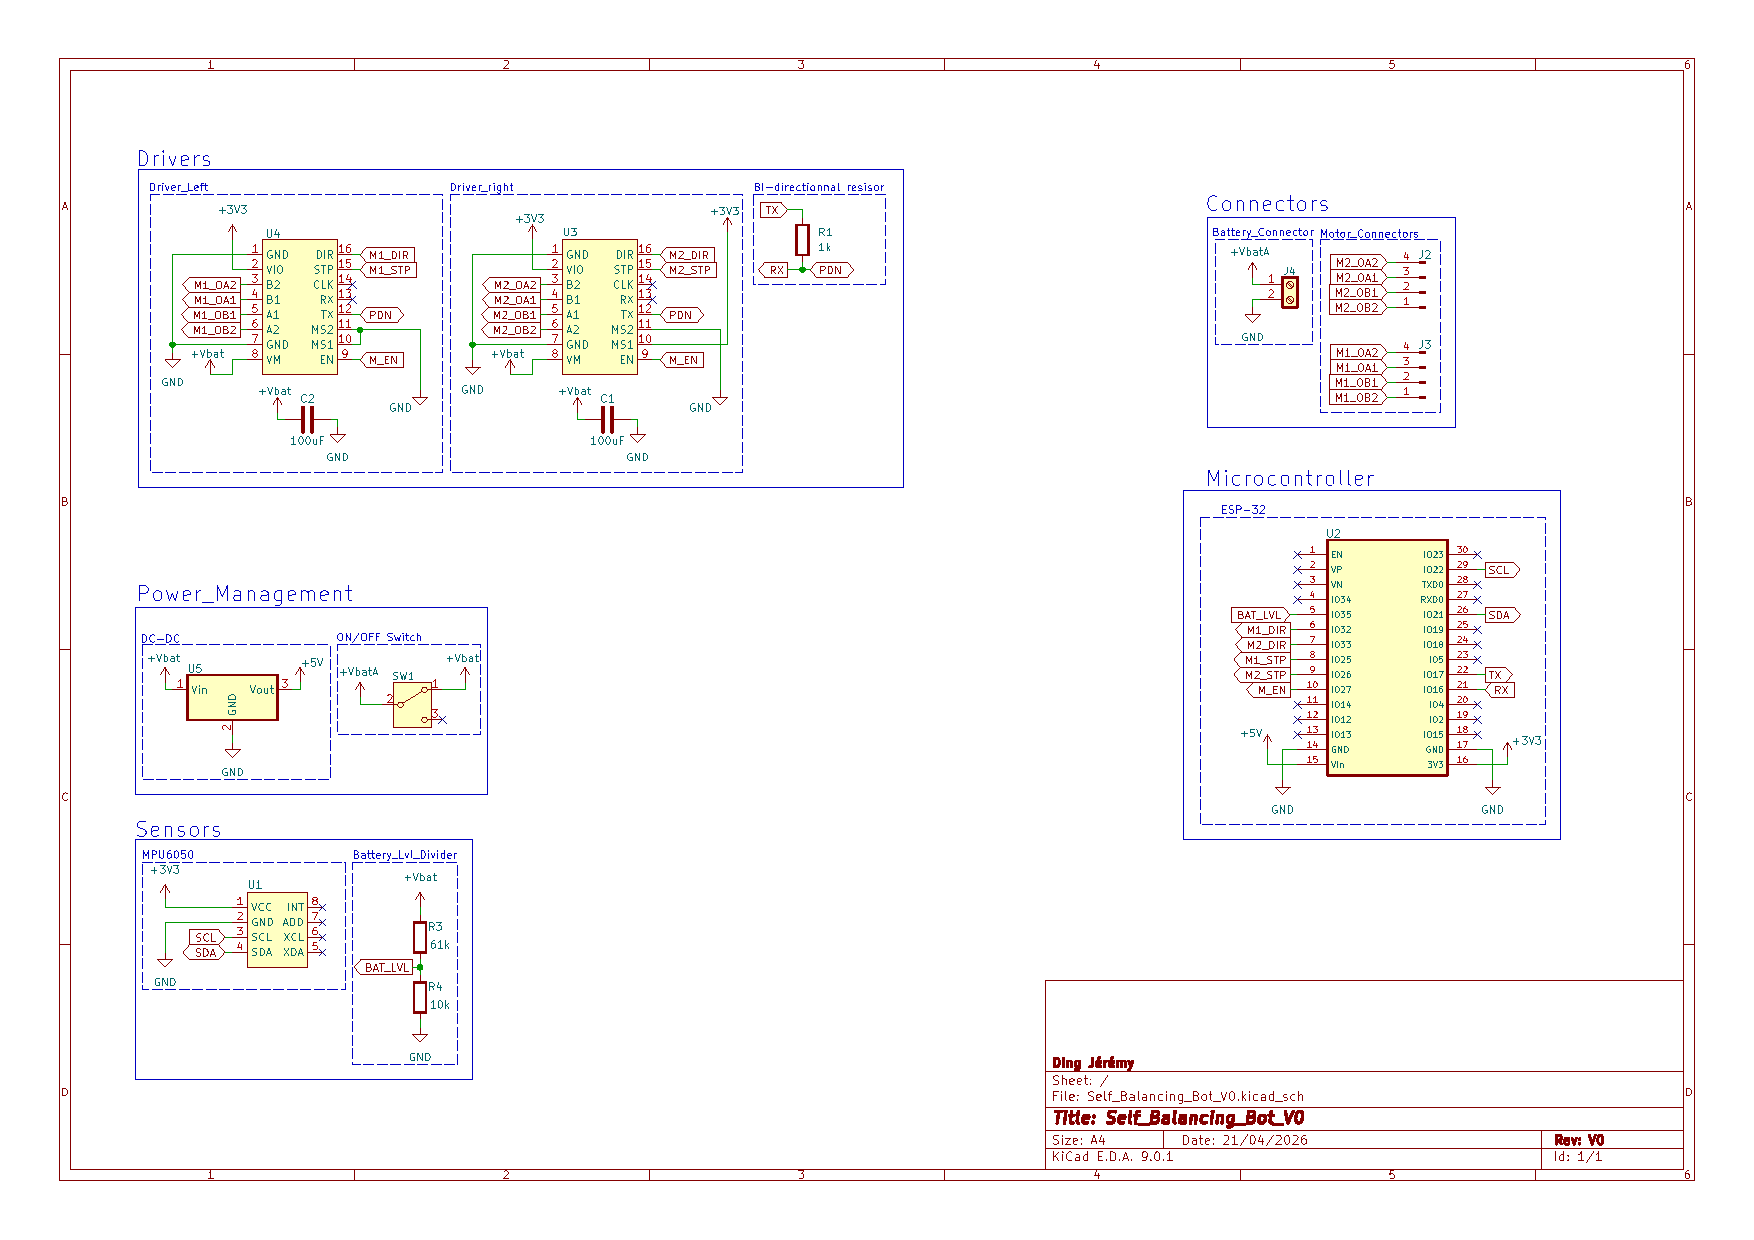
\includepdf[
    pages=-,
    fitpaper=true,
    pagecommand={\thispagestyle{plain}}
]{assets/figures/Self_Balancing_Bot_V0.pdf}

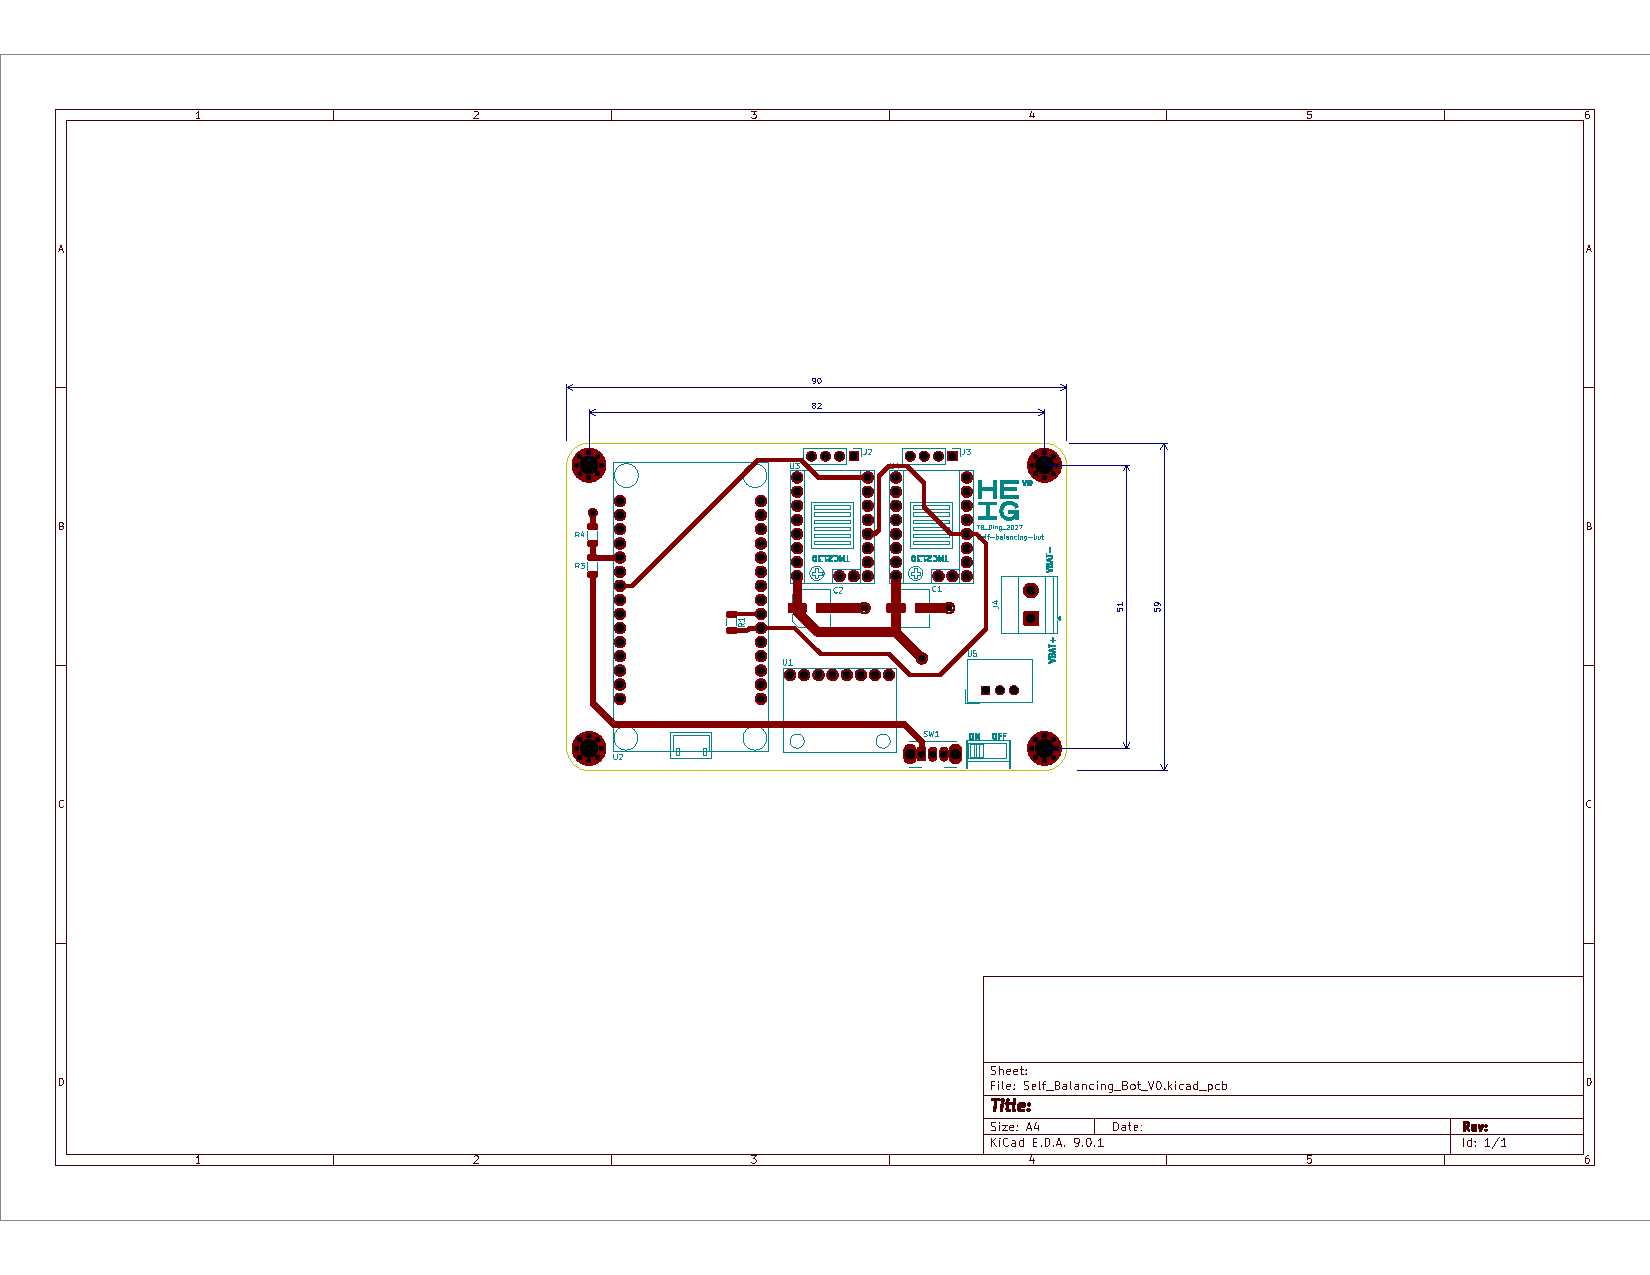
\includepdf[
    pages=-,
    fitpaper=true,
    pagecommand={\thispagestyle{plain}}
]{assets/figures/kicad_pcb_fcu.pdf}
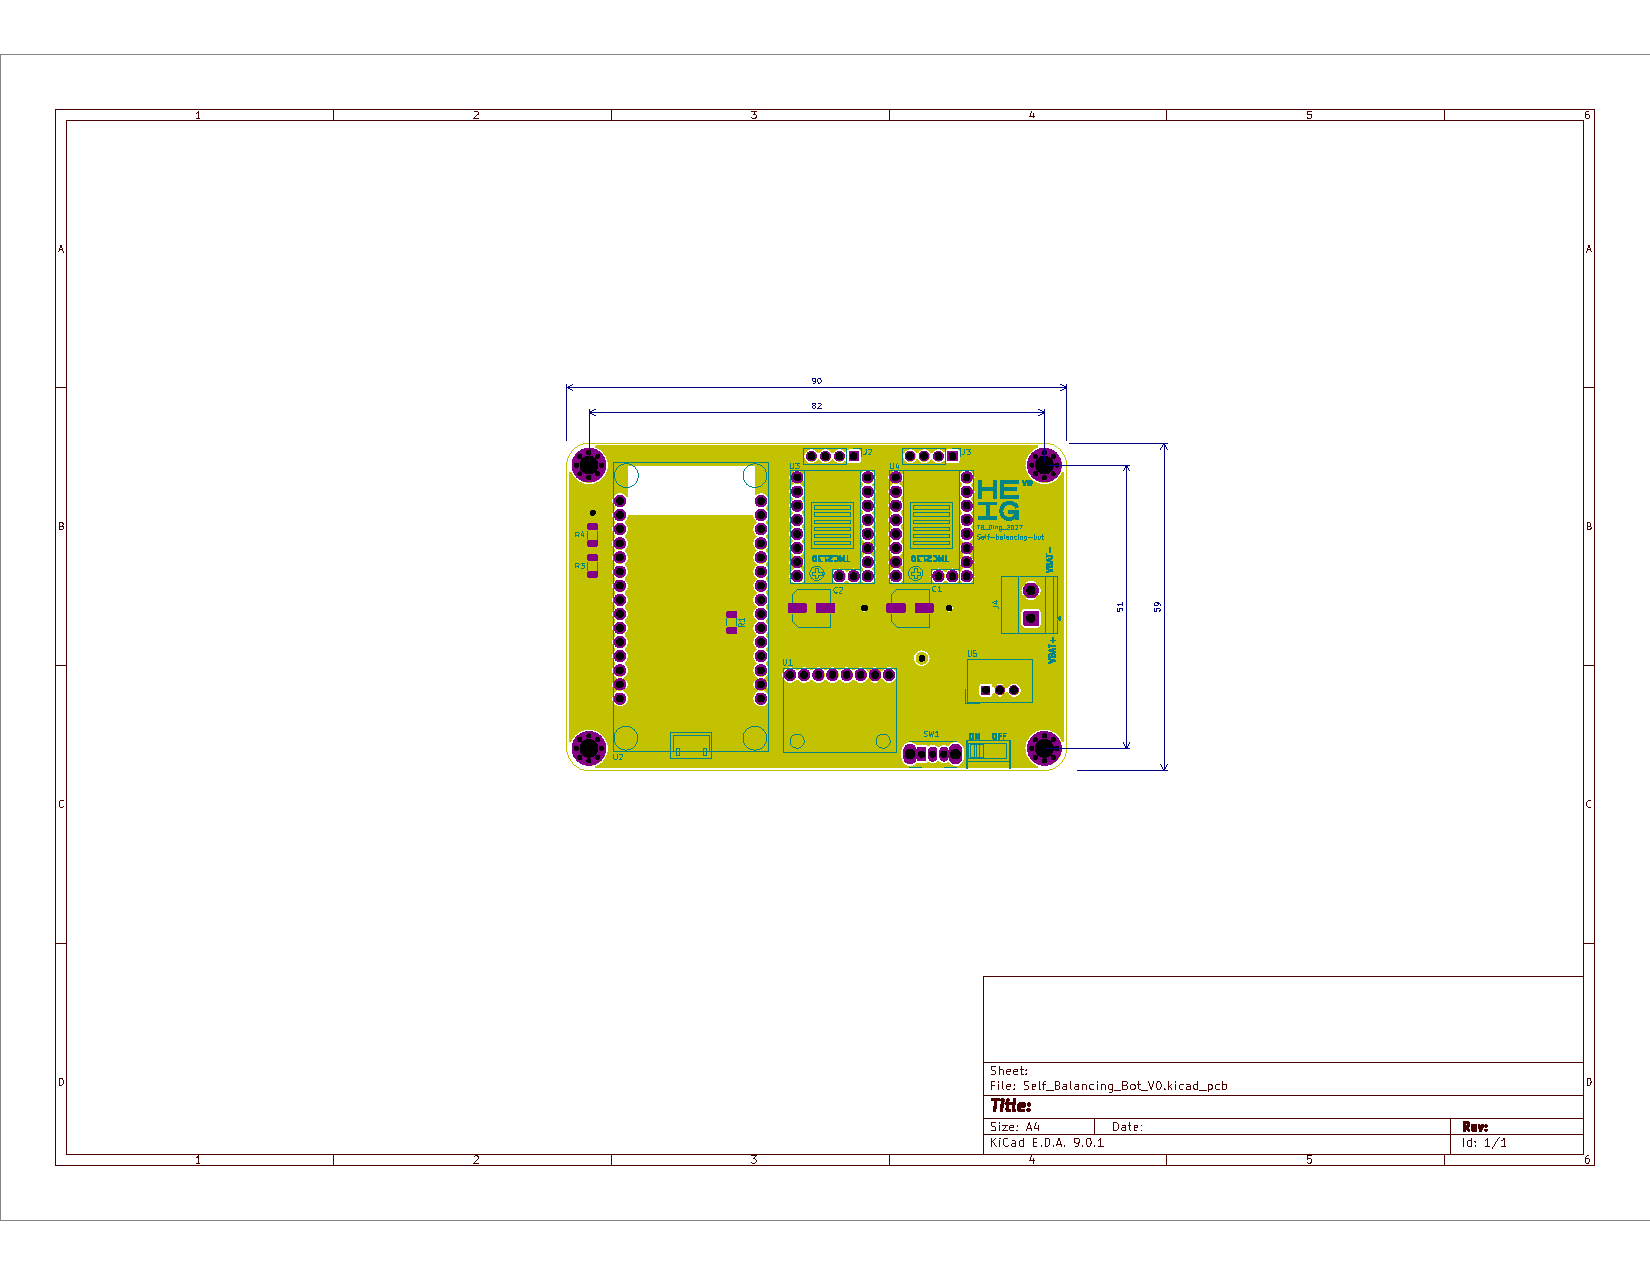
\includepdf[
    pages=-,
    fitpaper=true,
    pagecommand={\thispagestyle{plain}}
]{assets/figures/kicad_pcb_in1cu.pdf}
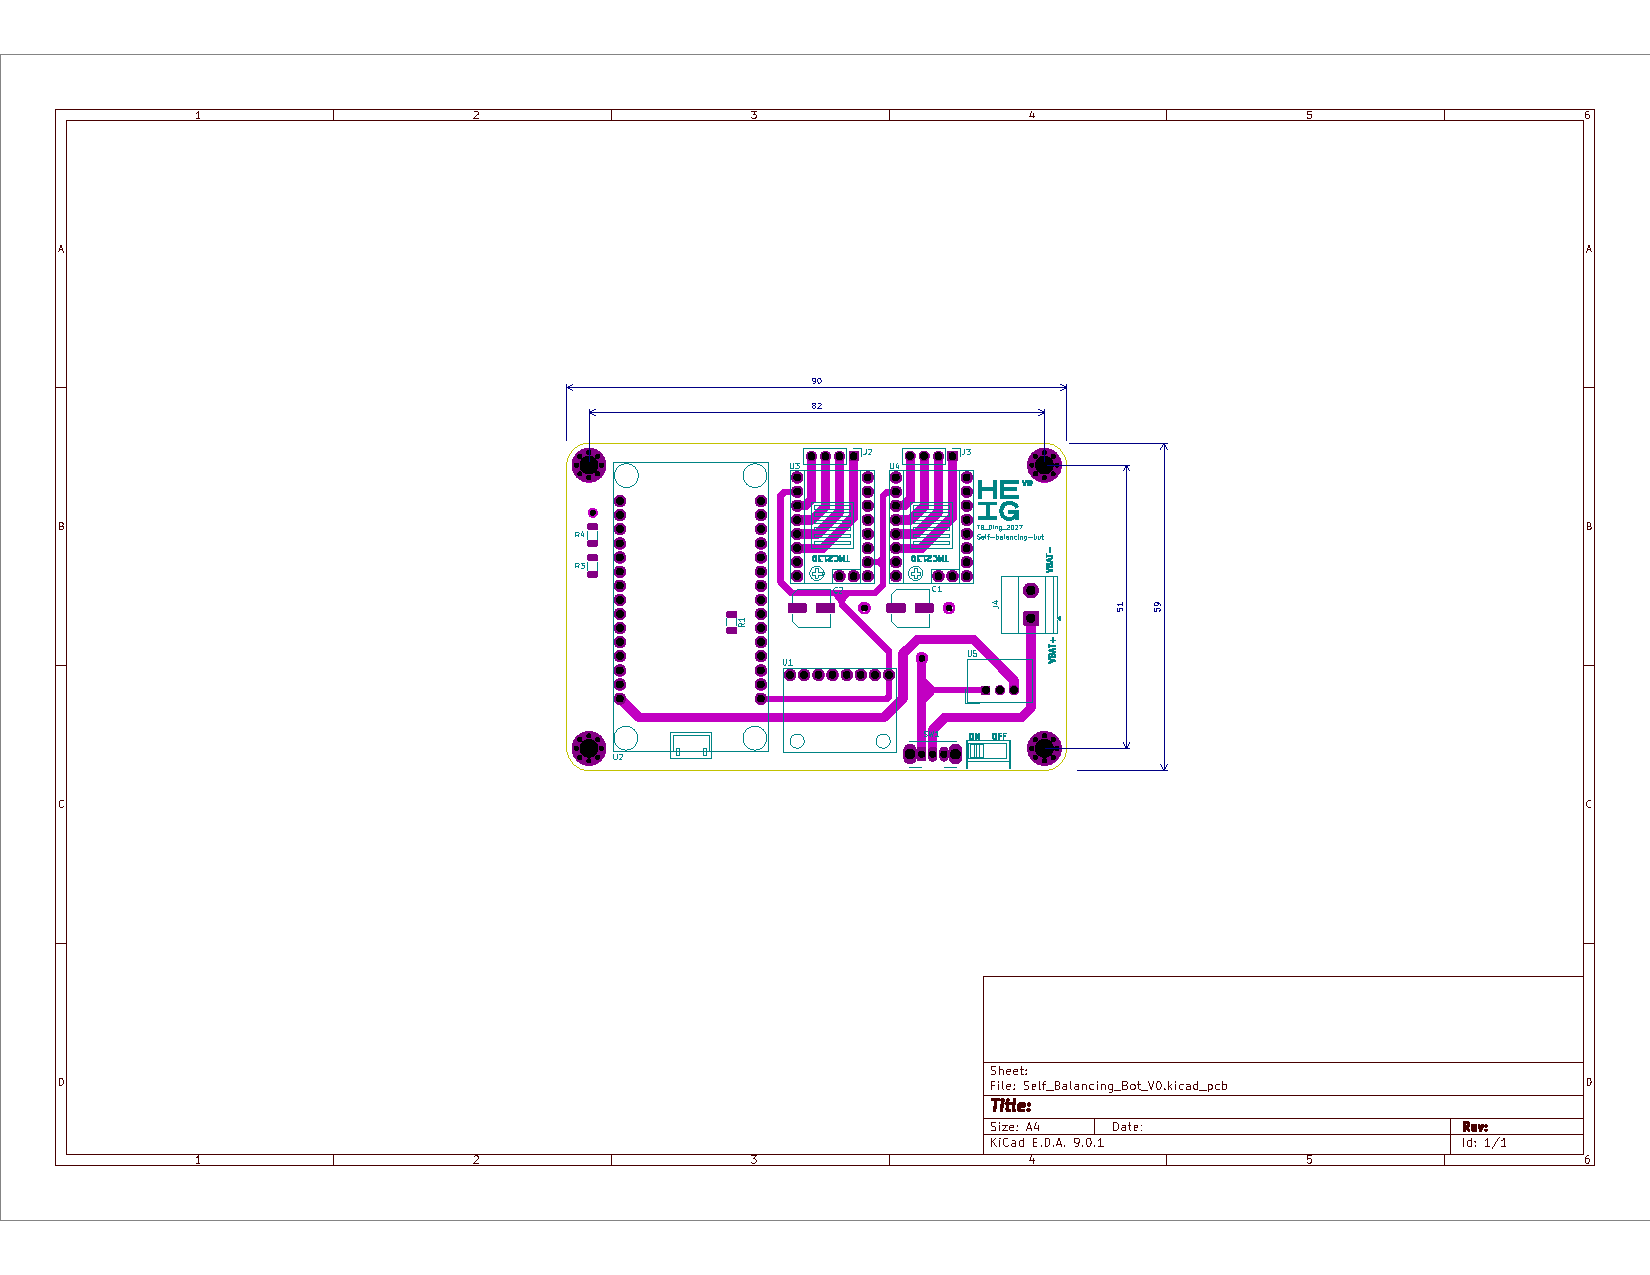
\includepdf[
    pages=-,
    fitpaper=true,
    pagecommand={\thispagestyle{plain}}
]{assets/figures/kicad_pcb_in2cu.pdf}
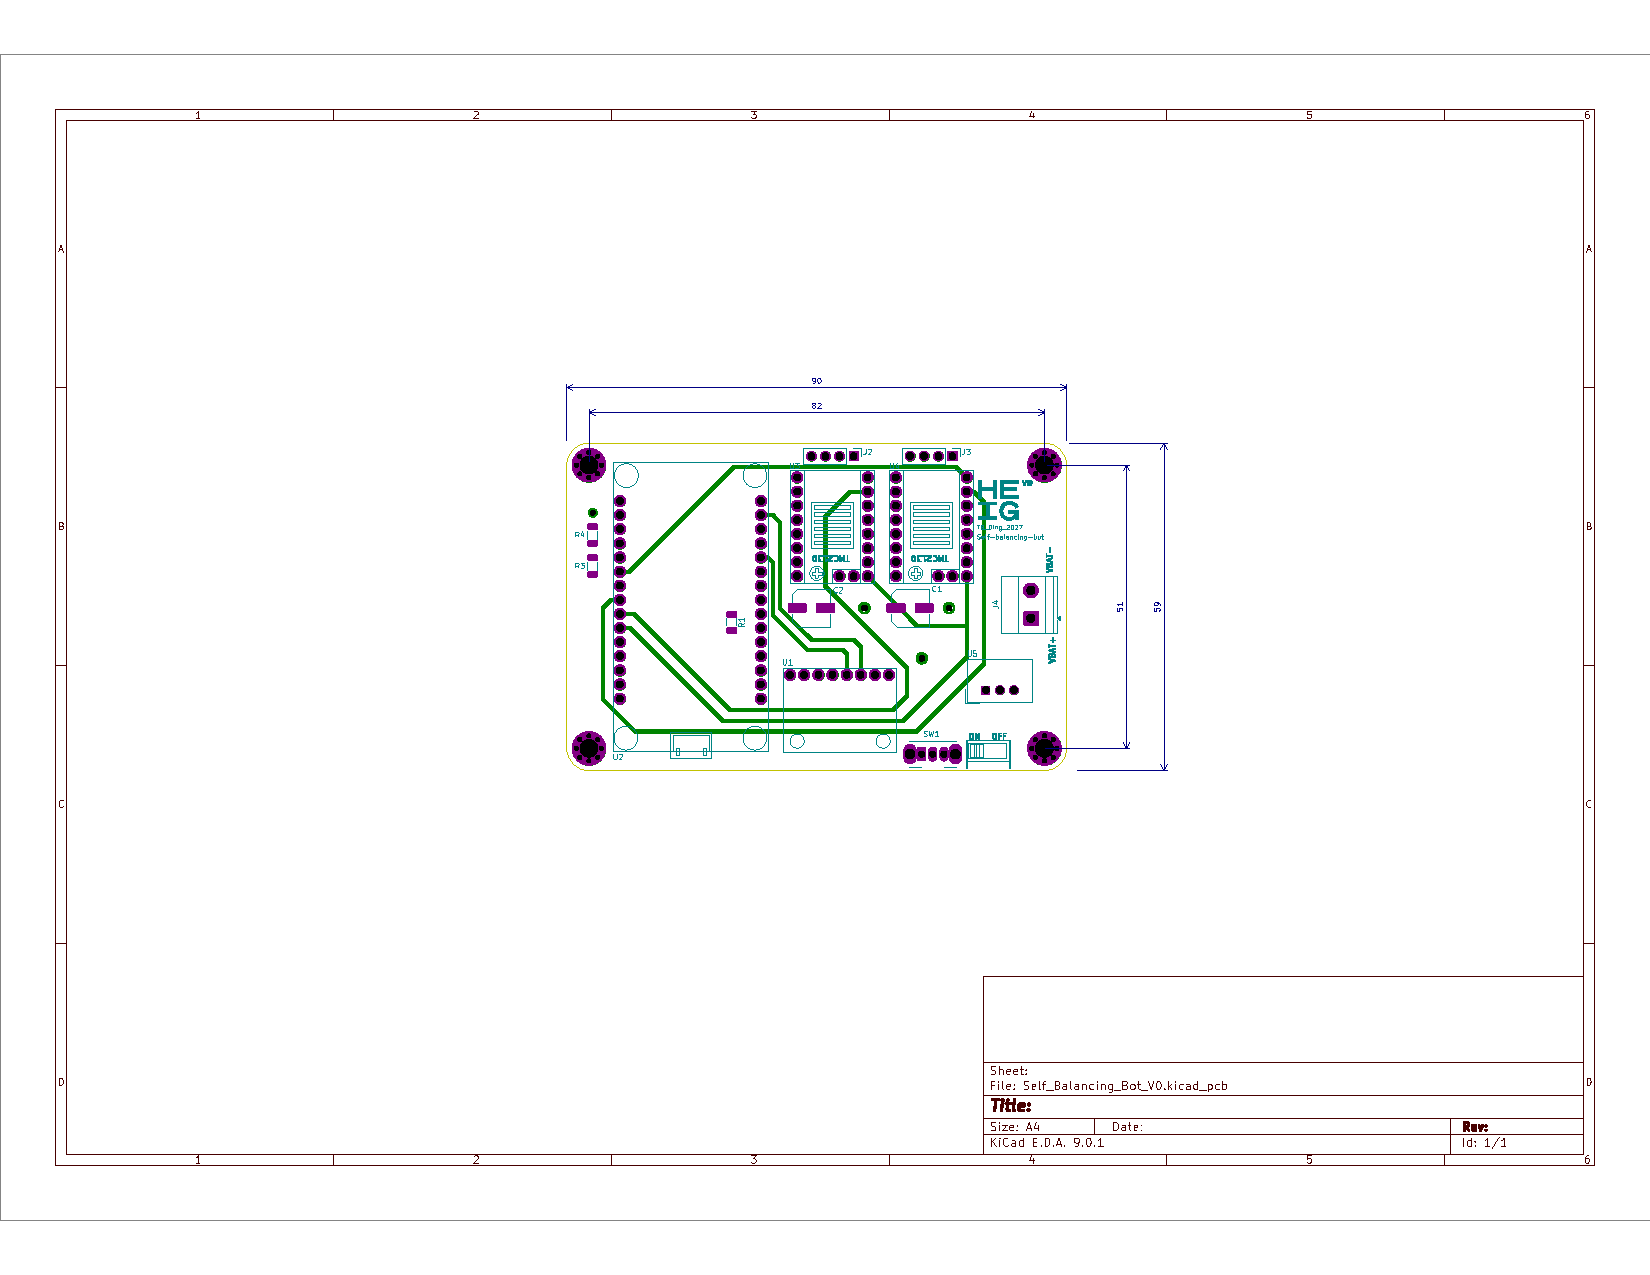
\includepdf[
    pages=-,
    fitpaper=true,
    pagecommand={\thispagestyle{plain}}
]{assets/figures/kicad_pcb_bcu.pdf}

%%fi

\let\cleardoublepage\clearpage
\backmatter

\label{glossaire}
\glsaddall[types=main]
\printglossary
\label{index}
\printindex

% Le colophon est le dernier élément d'un document qui contient des notes de l'auteur concernant la mise en page et l'édition du document : il est parfaitement optionnel.
\input{colophon.tex}

\end{document}
